\documentclass[aspectratio=169]{beamer}

\usefonttheme[stillsansserifmath]{serif}
\usepackage{graphicx}
\usepackage{amsfonts}
\usepackage{mathtools, nccmath}
\usepackage{amssymb, amsmath}
\usepackage{xspace}
\usepackage{tikz}
\usepackage{standalone}
\usepackage{euler}
\usepackage{color,xcolor}
\usepackage{fontspec}
\usepackage{nameref}
\usepackage{manfnt}
\usepackage{listings}
\usepackage{xcolor}
\usepackage{algorithm}
\usepackage[noend]{algpseudocode}
\usepackage{algorithmicx}
\usepackage{docs/style}

\usepackage{xepersian}
\settextfont{Yas}

% Persian specific
\newcommand{\itmsep}[1]{\raggedleft\setlength\itemsep{#1}}
\newcommand{\itemr}{\raggedleft\setlength\itemsep{3mm}}
\newcommand{\fn}[2]{\LR{\LTRfootnote[frame,#1]{~#2}}}
%\newcommand{\fn}[2]{{\LR{\footnote[frame,#1]{{~\LR{#2}}}}}}
\newcommand{\fnn}[1]{{\LR{\footnote[frame]{{~\LR{#1}}}}}}
\newcommand{\m}[1]{\ensuremath{\mathnormal{#1}}}
\newcommand{\mc}[1]{\ensuremath{\mathtt{#1}}}
\newcommand{\scl}{\ensuremath{\Sigma^*}\xspace}
\newcommand{\gcl}{\ensuremath{\Gamma^*}\xspace}
\newcommand{\gin}{\ensuremath{\mathnormal{\in}}\xspace}
%\newcommand{\gand}{\ensuremath{\mathnormal{\land}}\xspace}
\newcommand{\gand}{\&\&\xspace}
\newcommand{\alglr}{\LTR\ttfamily\small}
\newcommand{\st}[1]{\ensuremath{\mathnormal{\{#1\}}}\xspace}
\newcommand{\gst}[1]{\ensuremath{\mathnormal{\{\text{\texttt{#1}}\}}}\xspace}
\newcommand{\cpp}{C++\xspace}
\newcommand{\enc}[1]{\ensuremath{\mathnormal{\langle#1\rangle}}\xspace}
\newcommand{\abo}[1]{\ensuremath{\mathnormal{O(#1)}}\xspace}
\newcommand{\aso}[1]{\ensuremath{\mathnormal{o(#1)}}\xspace}
\newcommand{\aom}[1]{\ensuremath{\mathnormal{\Omega(#1)}}\xspace}
\newcommand{\ath}[1]{\ensuremath{\mathnormal{\Theta(#1)}}\xspace}
\newcommand{\dom}[2]{\ensuremath{\mathnormal{\Big[ \dfrac{#1}{#2} \Big]}}\xspace}

\newcommand{\Proc}[2]{\Statex \textbf{procedure} \textsc{#1}(#2)}
\newcommand{\Func}[2]{\Statex \textbf{function} \textsc{#1}(#2)}
\newcommand{\To}{\textbf{to}\xspace}
\newcommand{\Aand}{\textbf{and}\xspace}
\newcommand{\Aor}{\textbf{or}\xspace}



\newcommand\pro{\ensuremath{\rightarrow}\xspace}
\newcommand\der{\ensuremath{\Rightarrow}\xspace}
\newcommand\ders{\ensuremath{\stackrel{\mbox{*}}{\Rightarrow}}\xspace}
\newcommand{\dern}[1]{\ensuremath{\stackrel{\mbox{\small #1}}{\Rightarrow}}\xspace}
\newcommand\move{\ensuremath{\vdash}\xspace}
\newcommand\moves{\ensuremath{\stackrel{\small *}{\vdash}}\xspace}
\newcommand{\movesn}[1]{\ensuremath{\stackrel{\small *}{\vdash_{#1}}}\xspace}
\newcommand{\moven}[1]{\ensuremath{\mathnormal{\vdash_{#1}}}\xspace}

\newcommand{\code}[1]{{\LR{\texttt{#1}}}}
\newcommand{\txtlr}[1]{\text{\LR{#1}}}


% Abbreviations
\newcommand{\ie}{\latin{i.e.,~}}
\newcommand{\eg}{\latin{e.g.,~}}
\newcommand{\cf}{\latin{cf.~}}
\newcommand{\etal}{\latin{et al.~}}
\newcommand{\etc}{\unskip~\latin{etc.}\xspace}
\newcommand{\apriori}{\latin{a priori}}
\newcommand{\wrt}{\latin{w.r.t.~}}
%\newtheorem{theorem}{Theorem}

\newcommand\NN{\ensuremath{\mathbb{N}}\xspace}
\newcommand\RR{\ensuremath{\mathbb{R}}\xspace}
\newcommand\NNS{\ensuremath{\mathbb{N}^*}\xspace}
\newcommand\NNZ{\ensuremath{\mathbb{N}\backslash\{0\}}\xspace}
\newcommand\RRP{\ensuremath{\mathbb{R}^+}\xspace}
\newcommand\vect[1]{\ensuremath{\boldsymbol{\vec{#1}}}}
\newcommand\MP{\ensuremath{\mathcal{P}}\xspace}

\newcommand\de{\mathrel{\bullet\mkern-2.5mu{\rightarrow}}}
\newcommand\ue{\mathrel{\bullet\mkern-3mu{-}\mkern-3mu\bullet}}

\DeclareMathOperator*{\argmax}{arg\,max}
\DeclareMathOperator*{\argmin}{arg\,min}

\DeclareMathOperator{\lcm}{lcm}
\DeclareMathOperator{\Spec}{Spec}
\DeclareMathOperator{\Res}{Res}
%\DeclareMathOperator{\land}{and}

\newcommand{\fl}[1]{\ensuremath{\lfloor #1 \rfloor}}
\newcommand{\bfl}[1]{\ensuremath{\big\lfloor #1 \big\rfloor}}
\newcommand{\Bfl}[1]{\ensuremath{\Big\lfloor #1 \Big\rfloor}}
\newcommand{\bgfl}[1]{\ensuremath{\bigg\lfloor #1 \bigg\rfloor}}
\newcommand{\Bgfl}[1]{\ensuremath{\Bigg\lfloor #1 \Bigg\rfloor}}

\newcommand{\cl}[1]{\ensuremath{\lceil #1 \rceil}}
\newcommand{\bcl}[1]{\ensuremath{\big\lceil #1 \big\rceil}}
\newcommand{\Bcl}[1]{\ensuremath{\Big\lceil #1 \Big\rceil}}
\newcommand{\bgcl}[1]{\ensuremath{\bigg\lceil #1 \bigg\rceil}}
\newcommand{\Bgcl}[1]{\ensuremath{\Bigg\lceil #1 \Bigg\rceil}}

\newcommand{\mtx}[1]{\begin{pmatrix} #1 \end{pmatrix}}
\newcommand{\smtx}[1]{\begin{psmallmatrix} #1 \end{psmallmatrix}}

\definecolor{commentgreen}{RGB}{2,112,10}
\definecolor{eminence}{RGB}{108,48,130}
\definecolor{brightmaroon}{rgb}{0.76, 0.13, 0.28}
\definecolor{darkred}{rgb}{0.55, 0.0, 0.0}
\lstset {
    language=C++,
    frame=tb,
    tabsize=4,
    showstringspaces=false,
    numbers=left,
    %upquote=true,
    commentstyle=\color{commentgreen},
    keywordstyle=\color{eminence},
    stringstyle=\color{darkred},
    basicstyle=\small\ttfamily, % basic font setting
    emph={int,char,double,float,unsigned,long,short,void,bool},
    emphstyle={\color{blue}},
    %escapechar=\&,
    % keyword highlighting
    %classoffset=1, % starting new class
    %otherkeywords={>,<,.,;,-,!,=,~},
    %morekeywords={>,<,.,;,-,!,=,~},
    %keywordstyle=\color{weborange},
    %classoffset=0,
}

\makeatletter
\NewDocumentCommand{\LeftComment}{s m}{%
	\IfBooleanF{#1}{\hspace*{\ALG@thistlm}}\textcolor{commentgreen}{\(~\triangleright\) #2}}
\makeatother


\newenvironment{itemframe}[2]{
\begin{frame}[environment=itemframe]{#1}

\framesubtitle{\small \color{gray} \quad #2}
\itemize
\itemr

}{
\enditemize
\end{frame}
}

\newcommand{\centerimg}[2][.5]{
    \begin{figure}[h!]
        \centering
        \includegraphics[width=#1\textwidth]{#2}
    \end{figure}
}

\usetikzlibrary{arrows,calc}
\usetikzlibrary{positioning,shapes,chains,fit}


\tikzset{
    %Define style for boxes
    node/.style={
        circle,
        draw=black, thick,
        align=center,
    },
    ss/.style={
        circle,
        draw=black,
        align=center,
    },
    proc/.style={
        rounded corners,
        draw=black,
        align=center,
    },
    ifelse/.style={
	ellipse,
	draw=black,
	align=center,
    },
    cloudy/.style={
	cloud,
	cloud puffs=12,
	cloud ignores aspect,
	align=center,
	draw=black,
    },
    txt/.style={
        draw = none,
        align = center,
        font = \footnotesize,
    },
    coin/.style={
        rectangle,
        minimum height=1mm,
        minimum width=1cm,
        draw=black,
        fill=black!20,
        rounded corners
    },
    towercolor/.style={
        fill=black!80
    },
    towerbase/.style={
        trapezium,
        trapezium angle=75,
        trapezium stretches=true,
        towercolor,
        minimum width=7mm,
        minimum height=2mm,
    },
    tower/.style={
        rectangle,
        rounded corners,
        towercolor,
        minimum width=2mm,
        minimum height=26mm,
    },
    start-end/.style={
        draw,
        rectangle,
        rounded corners,
    },
    input/.style={ % requires library shapes.geometric
        draw,
        trapezium,
        trapezium left angle=60,
        trapezium right angle=120,
    },
    operation/.style={
        draw,
        rectangle
    },
    loop/.style={ % requires library shapes.misc
        draw,
        chamfered rectangle,
        chamfered rectangle xsep=2cm
    },
    decision/.style={ % requires library shapes.geometric
        draw,
        diamond,
        aspect=#1
    },
    decision/.default=1,
    print/.style={ % requires library shapes.symbols
        draw,
        tape,
        tape bend top=none
    },
    connection/.style={
        draw,
        circle,
        radius=5pt,
    },
    process rectangle outer width/.initial=0.15cm,
    predefined process/.style={
        rectangle,
        draw,
        append after command={
        \pgfextra{
          \draw
          ($(\tikzlastnode.north west)-(0,0.5\pgflinewidth)$)--
          ($(\tikzlastnode.north west)-(\pgfkeysvalueof{/tikz/process rectangle outer width},0.5\pgflinewidth)$)--
          ($(\tikzlastnode.south west)+(-\pgfkeysvalueof{/tikz/process rectangle outer width},+0.5\pgflinewidth)$)--
          ($(\tikzlastnode.south west)+(0,0.5\pgflinewidth)$);
          \draw
          ($(\tikzlastnode.north east)-(0,0.5\pgflinewidth)$)--
          ($(\tikzlastnode.north east)+(\pgfkeysvalueof{/tikz/process rectangle outer width},-0.5\pgflinewidth)$)--
          ($(\tikzlastnode.south east)+(\pgfkeysvalueof{/tikz/process rectangle outer width},0.5\pgflinewidth)$)--
          ($(\tikzlastnode.south east)+(0,0.5\pgflinewidth)$);
        }  
        },
        text width=#1,
        align=center
    },
    predefined process/.default=1.75cm,
    man op/.style={ % requires library shapes.geometric
        draw,
        trapezium,
        shape border rotate=180,
        text width=2cm,
        align=center,
    },
    extract/.style={
        draw,
        isosceles triangle,
        isosceles triangle apex angle=60,
        shape border rotate=90
    },
    merge/.style={
        draw,
        isosceles triangle,
        isosceles triangle apex angle=60,
        shape border rotate=-90
    },
}


\title{طراحی الگوریتم‌ها}
\author{
آرش شفیعی
}

\institute{
\\

\includegraphics[height=1.2cm]{logos/ui.png}
%\\
%دانشگاه اصفهان
}
\date{}

\begin{document}

\begin{frame}[plain]
\begin{center}
به نام خدا
\end{center}

\maketitle

%\begin{center}
%{\footnotesize arash.shafiei@gmail.com}
%\end{center}

\end{frame}
\setcounter{framenumber}{0}

%\input{docs/licence}

\raggedleft

%%%%%%%%%%%%
%\begin{frame}{فهرست مطالب}
%\begin{flushright}
%  \tableofcontents
%\end{flushright}
%\end{frame}
%%%%%%%%%%%%

%%%%%%%%%%%%
%%%%%%%%%%%%%%%%%%%%%%%%%
\section{الگوریتم‌های تقسیم و حل}
%%%%%%%%%%%%%%%%%%%%%%%%%


\begin{frame}{‌طراحی الگوریتم با استقرا}
\begin{itemize}\itemr
\item[-]
استقرای ریاضی
\fn{1}{induction}
روشی است برای اثبات درستی گزاره
\m{P(n)}
برای همه اعداد طبیعی
\m{n}
. به عبارت دیگر هنگامی که می‌خواهیم درستی گزاره‌های
\m{P(1)}
،
\m{P(2)}
،
\m{\cdots}
،
\m{P(n)}
را ثابت کنیم، می‌توانیم از استقرا استفاده کنیم.
\item[-]
به زبان استعاری با استفاده از استقرا ثابت می‌کنیم که می‌توانیم هر نردبانی را با طول دلخواه یا بینهایت بالا برویم اگر ثابت کنیم که می‌‌توانیم برروی پله اول برویم (پایهٔ استقرا
\fn{2}{base case}
) و همچنین ثابت کنیم اگر برروی پلهٔ
\m{n}
بودیم می‌توانیم برروی پله
\m{n+1}
نیز گام بگذاریم (گام استقرا
\fn{3}{induction step}
).
\item[-]
بنابراین در روش استقرایی برای اثبات درستی
\m{P(n)}
باید ثابت کنیم
\m{P(1)}
درست است (پایهٔ استقرا) و همچنین اگر
\m{P(n)}
درست باشد، آنگاه
\m{P(n+1)}
نیر درست است (گام استقرا).
\end{itemize}
\end{frame}


\begin{frame}{‌طراحی الگوریتم با استقرا}
\begin{itemize}\itemr
\item[-]
استقرای ریاضی براساس اصل دومینو
\fn{1}{domino principle}
است. فرض کنید تعداد زیادی دومینو به صورت ایستاده در کنار یکدیگر قرار گرفته‌اند و می‌خواهیم همهٔ دومینوهای ایستاده را بیاندازیم. برای اینکه همهٔ دومینوها بر زمین بیفتند کافی است دومینوها به گونه‌ای قرار داده شوند که با افتادن اولین دومینو، دومین دومینو برزمین بیافتد و با افتادن دومی، سومی و به همین ترتیب با افتادن
\m{n}
امین دومینو،
\m{n+1}
امین دومینو بر زمین بیافتد. سپس کافی است به اولین دومینو ضربه‌ای بزنیم تا همه دومینوهای ایستاده بیافتند و نیازی به انداختن تک‌تک آنها نداریم.
\end{itemize}
\end{frame}

\iffalse
\begin{frame}{‌طراحی الگوریتم با استقرا}
\begin{itemize}\itemr
\item[-]
در طراحی یک مسئله به روش استقرایی، باید برای پاسخ مسئله یک رابطه پیدا کنیم و پاسخ مسئله را به روش استقرایی اثبات کنیم. و سپس می‌توانیم از رابطهٔ به دست آمده برای حل مسئله استفاده کنیم.
\item[-]
برای مثال فرض کنید می‌خواهیم جمع
\m{n}
عدد اول صحیح را به دست آوریم. برای این کار
\m{n}
عدد را با یکدیگر جمع کنیم. پس الگوریتم در واقع
\m{O(n)}
است.
\item[-]
برای حل این مسئله به روش استقرایی باید رابطه‌ای برای جواب مسئله پیدا کنیم. به عبارت دیگر آیا عبارتی وجود دارد که توسط آن بتوان جمع
\m{n}
عدد اول اعداد صحیح را به دست آورد؟
\end{itemize}
\end{frame}
\fi

\begin{frame}{‌طراحی الگوریتم با استقرا}
\begin{itemize}\itemr
\item[-]
برای مثال با استفاده از استقرا می‌توان اثبات کرد:
\begin{align*}
\m{P(n) = 1 + 2 + 3 + \cdots + n = \frac{n(n+1)}{2}}
\end{align*}
\item[-]
باید اثبات کنیم
\m{P(1) = \frac{1(2)}{2}}
درست است (پایهٔ استقرا) و همچنین اگر
\m{P(n) = \frac{n(n+1)}{2}}
باشد آنگاه
\m{P(n+1) = \frac{(n+1)(n+2)}{2}}
نیز درست است (گام استقرا).
\end{itemize}
\end{frame}


\begin{frame}{‌طراحی الگوریتم با استقرا}
\begin{itemize}\itemr
\item[-]
اثبات : 
\item[-]
پایه استقرا درست است زیرا 
\m{P(1) = 1 = \frac{1(2)}{2} = 1}
\item[-]
می‌دانیم
\m{P(n+1) = P(n) + (n+1)}
بنابراین
\m{P(n+1) = \frac{n(n+1)}{2} + (n+1)} .
با بسط این رابطه به دست می‌آوریم
\m{P(n+1) = \frac{(n+1)(n+2)}{2}} .
بنابراین گام استقرا نیز درست است.
\item[-]
با استفاده از این رابطه برای محاسبهٔ
\m{n}
عدد کافی است از رابطه
\m{P(n)}
استفاده کنیم. این الگوریتم در زمان
\m{O(1)}
انجام می‌شود، در حالی که جمع 
\m{n}
عدد با استفاده از یک حلقه در زمان
\m{O(n)}
انجام می‌شود.
\end{itemize}
\end{frame}



\begin{frame}{‌طراحی الگوریتم با استقرا}
\begin{itemize}\itemr
\item[-]
استقرای ریاضی در طراحی الگوریتم‌ها بسیار پر استفاده است.
\item[-]
برای طراحی یک الگوریتم برای حل یک مسئله با استفاده از استقرا کافی است :
\item[۱.]
مسئله را در حالت پایه یعنی حالتی که اندازه ورودی کوچک است حل کنیم.
\item[۲.]
نشان‌دهیم چگونه می‌توان یک مسئله را با استفاده از یک زیر مسئله (یعنی مسئله‌ای با اندازهٔ کوچک‌تر) حل کرد.
\end{itemize}
\end{frame}


\begin{frame}{‌طراحی الگوریتم با استقرا}
\begin{itemize}\itemr
\item[-]
فرض کنید می‌خواهیم به ازای دنباله‌ای از اعداد حقیقی
\m{a_0}
،
\m{a_1}
،
\m{a_2}
،
\m{\cdots}
،
\m{a_n}
و عدد داده شده
\m{x}،
مقدار چند جمله‌ای زیر را محاسبه کنیم.\\
\begin{align*}
\m{P_n(x) = a_nx^n + a_{n-1}x^{n-1} + \cdots + a_1x + a_0}
\end{align*}
\end{itemize}
\end{frame}


\begin{frame}{‌طراحی الگوریتم با استقرا}
\begin{itemize}\itemr
\item[-]
یک الگوریتم بدیهی برای حل این مسئله با جایگذاری اعداد
\m{a_i}
و
\m{x}
در چند جمله
\m{P_n(x)}
مقدار آن را محاسبه می‌کند.
\begin{algorithm}[H]\alglr
\caption{Compute Polynomial}
  \begin{algorithmic}[1]
   \Func{ComputePolynomial}{a[], x}
    \State P = a[0]
    \For{i = 1 to n}
      \State X = 1
      \For{j = 1 to i}
          \State X = X * x
       \EndFor
       \State P = P + a[i] * X
     \EndFor
     \State \Return P                          
  \end{algorithmic}
  \label{alg:merge}
\end{algorithm}
\item[-]
پیچیدگی زمانی این الگوریتم
\m{O(n^2)}
است.
\item[-]
حال می‌خواهیم با استفاده از استقرا این مسئله را در زمان کمتری حل کنیم.
\end{itemize}
\end{frame}


\begin{frame}{‌طراحی الگوریتم با استقرا}
\begin{itemize}\itemr
\item[-]
برای حل مسئله با استفاده از استقرا باید بتوانیم مسئله را بر اساس یک زیر مسئله بیان کنیم.
\item[-]
یک زیر مسئله از مسئلهٔ محاسبه چند جمله‌ای را به صورت زیر در نظر بگیرید.
\begin{align*}
\m{P_{n-1}(x) = a_nx^{n-1} + a_{n-1}x^{n-2} + \cdots + a_1}
\end{align*}
\item[-]
فرض کنید جواب
\m{P_{n-1}(x)}
داده شده است. چگونه می‌توانیم
\m{P_n(x)}
را محاسبه کنیم؟
\end{itemize}
\end{frame}


\begin{frame}{‌طراحی الگوریتم با استقرا}
\begin{itemize}\itemr
\item[-]
برای محاسبه
\m{P_n(x)}
می‌توانیم رابطه‌ای به صورت زیر بنویسیم.
\begin{align*}
\m{P_n(x) = x \cdot P_{n-1}(x) + a_0}
\end{align*}
\item[-]
همچنین می‌توانیم
\m{P_{n-1}(x)}
را بر اساس
\m{P_{n-2}(x)}
محاسبه کنیم.
\item[-]
داریم :
\begin{align*}
\m{P_{n-2}(x) = a_nx^{n-2} + a_{n-1}x^{n-3} + \cdots + a_2}
\end{align*}
\item[-]
بنابراین خواهیم داشت :
\begin{align*}
\m{P_{n-1}(x) = x \cdot P_{n-2}(x) + a_1}
\end{align*}
\end{itemize}
\end{frame}


\begin{frame}{‌طراحی الگوریتم با استقرا}
\begin{itemize}\itemr
\item[-]
در حالت کلی برای محاسبه
\m{P_{n-j}(x)}
با استفاده از یک زیرمسئله می‌توانیم رابطهٔ زیر را ارائه کنیم:
\begin{align*}
\m{P_{n-j}(x) = x \cdot P_{n-(j+1)}(x) + a_j}
\end{align*}
\item[-]
در حالت پایه داریم:
\begin{align*}
\m{P_0(x) = a_n}
\end{align*}
\end{itemize}
\end{frame}


\begin{frame}{‌طراحی الگوریتم با استقرا}
\begin{itemize}\itemr
\item[-]
فرض کنیم
\m{n - j = i}
، در اینصورت خواهیم داشت :
\begin{align*}
\left\{ \begin{array}{lcl}
\m{P_i(x) = x \cdot P_{i-1}(x) + a_{n-i}} & \m{i > 0} & \text{اگر} \\
\m{P_0(x) = a_n} & \m{i = 0} & \text{اگر}
\end{array}\right.
\end{align*}
\end{itemize}
\end{frame}


\begin{frame}{‌طراحی الگوریتم با استقرا}
\begin{itemize}\itemr
\item[-]
بنابراین با استفاده از رابطه بازگشتی به دست آمده می‌توانیم الگوریتمی به صورت زیر بنویسیم.
\begin{algorithm}[H]\alglr
\caption{Compute Polynomial}
  \begin{algorithmic}[1]
   \Func{ComputePolynomial}{a[], x}
    \State P = a[n]
    \For{i = 1 to n}
       \State P = x * P + a[n-i]
     \EndFor  
     \State \Return P                           
  \end{algorithmic}
  \label{alg:merge}
\end{algorithm}
\item[-]
پیچیدگی زمانی این الگوریتم
\m{O(n)}
است که از الگوریتم بدیهی که در زمان
\m{O(n^2)}
چند جمله‌ای را محاسبه می‌کند سریع‌تر است.
\end{itemize}
\end{frame}


\begin{frame}{‌طراحی الگوریتم با استقرا}
\begin{itemize}\itemr
\item[-]
این الگوریتم به روش هورنر
\fn{1}{Horner's method}
معروف است که توسط ریاضی‌دان انگلیسی ویلیام هورنر
\fn{2}{William Horner}
ابداع شده است، گرچه خود هورنر آن را به ریاضی‌دان فرانسوی-ایتالیایی ژوزف لاگرانژ
\fn{3}{Joseph-Louis Lagrange}
نسبت داده است. گفته می‌شود این الگوریتم قبل از لاگرانژ احتمالاً توسط ریاضی‌دانان ایرانی و چینی ابداع شده است.
\begin{align*}
&\m{a_0 + a_1x + a_2x^2 + \cdots + a_nx^n =} \\
&~~~~~~~~~~~~~~~~~~~~~~~~~~~~~~~\m{a_0 + x ( a_1 + x (a_2 + x ( a_3 + \cdots + x (a_{n-1} + xa_n) \cdots)))}
\end{align*}
\end{itemize}
\end{frame}
\begin{frame}{‌الگوریتم‌های تقسیم و حل}
\begin{itemize}\itemr
\item[-]
برای حل یک مسئله به روش‌های متنوعی می‌توان الگوریتم طراحی کرد.
\item[-]
الگوریتم مرتب‌سازی درجی یک الگوریتم ساده است که به روش افزایشی با مرتب‌سازی زیر آرایه‌های کوچک‌تر آرایه آغاز می‌شود و در نهایت کل آرایه را مرتب می‌کند. در واقع به ازای هر عنصر
\code{A[i]}
، این عنصر در مکان مناسب خود در زیر آرایه مرتب شدهٔ
\code{A[1 : i-1]}
قرار می‌گیرد.
\end{itemize}
\end{frame}


\begin{frame}{‌الگوریتم‌های تقسیم و حل}
\begin{itemize}\itemr
\item[-]
در این قسمت با روشی دیگر برای حل مسئله‌های محاسباتی آشنا می‌شویم، که به آن روش تقسیم و حل
\fn{1}{divide and conquer method}
(تقسیم و غلبه)
گفته می‌شود و الگوریتم‌هایی که از این روش استفاده می‌کنند، در دستهٔ الگوریتم‌های تقسیم و حل قرار می‌گیرند.
\item[-]
از روش تقسیم و حل برای حل مسئلهٔ مرتب‌سازی استفاده می‌کنیم و زمان اجرای آن را محاسبه می‌کنیم.
\item[-]
خواهیم دید که با استفاده از این روش، مسئلهٔ مرتب‌سازی در زمان کمتری نسبت به الگوریتم مرتب‌سازی درجی حل می‌شود.
\end{itemize}
\end{frame}


\begin{frame}{‌الگوریتم‌های تقسیم و حل}
\begin{itemize}\itemr
\item[-]
بسیاری از  الگوریتم‌های کامپیوتری بازگشتی
\fn{1}{recursive}
هستند. در یک الگوریتم بازگشتی، برای حل یک مسئله با یک ورودی معین ، خود الگوریتم با ورودی‌های کوچکتر فراخوانی می‌شود.
\item[-]
برای مثال، برای به دست آوردن فاکتوریل عدد n کافی است فاکتوریل عدد n-1 را فراخوانی کنیم.
\item[-]
به الگوریتم‌هایی که ورودی مسئله را تقسیم می‌کنند و به طور بازگشتی الگوریتم را برای قسمت‌های تقسیم شده فراخوانی می‌‌کنند، الگوریتم‌های تقسیم و حل گفته می‌شود.
\end{itemize}
\end{frame}


\begin{frame}{‌الگوریتم‌های تقسیم و حل}
\begin{itemize}\itemr
\item[-]
به عبارت دیگر یک الگوریتم تقسیم و حل یک مسئله را به چند زیر مسئله تقسیم می‌کند که مشابه مسئلهٔ اصلی هستند و الگوریتم را برای زیر مسئله‌ها فراخوانی می‌کند و سپس نتایج به دست آمده از زیر مسئله‌ها را با هم ترکیب می‌کند تا نتیجهٔ نهایی برای مسئلهٔ اصلی به دست آید.
\item[-]
معمولاً‌ پس از شکسته شدن یک مسئله به زیر مسئله‌ها، زیر مسئله‌هایی به دست می‌آیند که می‌توانند دوباره شکسته شوند و این روند تا جایی ادامه پیدا می‌کند که مسئله امکان شکسته شدن نداشته باشد. وقتی مسئله امکان شکسته شدن نداشته باشد، حالت پایه
\fn{1}{base case}
به دست می‌آید که حل مسئله در حالت پایه به سادگی امکان پذیر است.
\end{itemize}
\end{frame}


\begin{frame}{‌الگوریتم‌های تقسیم و حل}
\begin{itemize}\itemr
\item[-]
یک الگوریتم تقسیم و حل از سه مرحلهٔ زیر تشکیل شده‌است.\\
1. تقسیم
\fn{1}{divide}
: مسئله به چند زیر مسئله که نمونه‌های کوچکتر مسئلهٔ اصلی هستند تقسیم می‌شود.\\
۲. حل یا غلبه
\fn{2}{conquer}
: زیر مسئله‌ها به صورت بازگشتی حل می‌شوند.\\
۳. ترکیب
\fn{3}{combine}
: زیر مسئله‌های حل شده با یکدیگر ترکیب می‌شوند تا جواب مسئلهٔ اصلی به دست بیاید.
\end{itemize}
\end{frame}


\begin{frame}{‌مرتب‌سازی ادغامی}
\begin{itemize}\itemr
\item[-]
الگوریتم مرتب‌سازی ادغامی
\fn{1}{merge sort}
در دستهٔ الگوریتم‌های تقسیم و حل قرار می‌گیرد. با شروع از آرایهٔ
\code{A[1:n]}
، در هر مرحله یکی از زیر آرایه‌های
\code{A[p:r]}
مرتب می‌شود و سپس این زیر آرایه‌ها با یکدیگر ادغام می‌شوند تا آرایهٔ اصلی مرتب شود. برای هر یک از زیر آرایه‌ها، الگوریتم مرتب‌سازی ادغامی فراخوانی می‌شود و به همین نحو، آن زیر آرایه‌ها تقسیم شده و به روش بازگشتی مرتب می‌شوند.
\end{itemize}
\end{frame}


\begin{frame}{‌مرتب‌سازی ادغامی}
\begin{itemize}\itemr
\item[-]
مراحل انجام مرتب‌سازی ادغامی به صورت زیر است :
\item[۱.]
تقسیم : آرایهٔ
\code{A[p:r]}
به دو زیرآرایهٔ مساوی تقسیم می‌شود. اگر 
\code{q} 
وسط 
\code{p}
 و 
\code{r}
  باشد، آنگاه دو آرایهٔ به دست آمده عبارتند از
\code{A[p:q]}
و
\code{A[q+1:r]}
. در مرحلهٔ اول 
\code{p}
 برابر با 
\code{1}
  و 
\code{r}
   برابر است با 
\code{n} .
\item[۲.]
حل : الگوریتم به صورت بازگشتی برای دو زیر آرایهٔ
\code{A[p:q]}
و
\code{A[q+1:r]}
فراخوانی می‌شود.
\item[۳.]
ترکیب : با ادغام دو آرایهٔ
\code{A[p:q]}
و
\code{A[q+1:r]}
که هر دو مرتب شده هستند، آرایهٔ مرتب شدهٔ
\code{A[p:r]}
به دست می‌آید.
\end{itemize}
\end{frame}


\begin{frame}{‌مرتب‌سازی ادغامی}
\begin{itemize}\itemr
\item[-]
این الگوریتم به طور بازگشتی فراخوانی می‌شود تا به حالت پایه برسیم.
در حالت پایه، آرایهٔ به دست آمده شامل تنها یک عنصر است که در این حالت آرایه نیاز به مرتب‌سازی ندارد. در واقع هنگامی به حالت پایه می‌رسیم که 
\code{p}
 برابر با 
\code{r}
  باشد.
\item[-]
در مرحلهٔ ادغام، با فرض اینکه دو آرایهٔ به دست آمده مرتب شده هستند، دو آرایه باید به نحوی با یکدیگر ترکیب شوند که آرایهٔ به دست آمده مرتب شده باشد.
\end{itemize}
\end{frame}


\begin{frame}{‌مرتب‌سازی ادغامی}
\begin{itemize}\itemr
\item[-]
الگوریتم مرتب‌سازی ادغامی به صورت زیر است.
\begin{algorithm}[H]\alglr
  \caption{Merge Sort} 
  \begin{algorithmic}[1]
    \Func{Merge-Sort}{A, p, r}
    \If{p >= r}	\LeftComment{zero or one element?}
    	\State \Return
    \EndIf    
    \State q = $\lfloor$ (p+r)/2 $\rfloor$	\LeftComment{ midpoint of A[p:r]}
    \State Merge-Sort (A, p, q)	\LeftComment{ recursively sort A[p:q]}
    \State Merge-Sort (A, q+1, r)	\LeftComment{ recursively sort A[q+1:r]}
    \State Merge (A, p, q, r) \LeftComment{Merge A[p:q] and A[q+1:r] into A[p:r].}
  \end{algorithmic}
  \label{alg:merge-sort}
\end{algorithm}
\end{itemize}
\end{frame}

\begin{frame}{‌مرتب‌سازی ادغامی}
\begin{itemize}\itemr
\item[-]
برای ادغام دو زیرآرایه از الگوریتم زیر استفاده می‌کنیم.
\begin{algorithm}[H]\alglr
  \caption{Merge Sort} 
  \begin{algorithmic}[1]
    \Func{Merge}{A, p, q, r}
    \State nl = q - p + 1 \LeftComment{ length of A[p:q]}
    \State nr = r - q \LeftComment{ length of A[q+1 : r]}
    \State let L[ 0 : nl - 1 ] and R[ 0 : nr - 1 ] be new arrays
    \For{i = 0 \To nl - 1} \LeftComment{ copy A[p:q] into L[0:nl - 1]}
      \State L[i] = A[p+i]
    \EndFor
    \For{j = 0 to nr - 1} \LeftComment{copy A[q+1:r] into L[0:nr - 1]} 
      \State R[j] = A[q + j + 1]
     \EndFor
  \end{algorithmic}
  \label{alg:merge}
\end{algorithm}
\end{itemize}
\end{frame}


\begin{frame}{‌مرتب‌سازی ادغامی}
\begin{itemize}\itemr
\item[-]
\begin{algorithm}[H]\alglr
  \caption{Merge Sort} 
  \begin{algorithmic}[1]
  \setcounter{ALG@line}{7}
    \Func{Merge}{A, p, q, r}
      \State i = 0 \LeftComment{ i indexes the smallest remaining element in L}
      \State j = 0 \LeftComment{j indexes the smallest remaining element in R}
      \State k = p \LeftComment{ k indexes the location in A to fill}
    \newline\LeftComment{ As long as each of the arrays L and R contains un unmerged element, copy the smallest unmerged element back into A[p : r].}                              
    \While{ i < nl \Aand j < nr}
          \If {L[i] <= R[j]}
              \State A[k] = L[i]
              \State i = i + 1
          \Else 
              \State A[k] = R[j]
              \State j = j + 1
           \EndIf
          \State k = k + 1
      \EndWhile
  \end{algorithmic}
  \label{alg:merge}
\end{algorithm}
\end{itemize}
\end{frame}



\begin{frame}{‌مرتب‌سازی ادغامی}
\begin{itemize}\itemr
\item[-]
\begin{algorithm}[H]\alglr
  \caption{Merge Sort} 
  \begin{algorithmic}[1]
    \setcounter{ALG@line}{18}
    \Func{Merge}{A, p, q, r}
    \newline\LeftComment{ Having gone through one of L and R entirely, copy the  remainder of the other to the end of A[p:r]}                                    
    \While{i < nl}
             \State A[k] = L[i]
             \State i = i + 1
             \State k = k + 1
     \EndWhile      
    \While{ j < nr}
            \State A[k] = R[j]
            \State j = j + 1
            \State k = k + 1 
      \EndWhile                                             
  \end{algorithmic}
  \label{alg:merge}
\end{algorithm}
\end{itemize}
\end{frame}


\begin{frame}{‌مرتب‌سازی ادغامی}
\begin{itemize}\itemr
\item[-]
یک مثال از ادغام دو زیر آرایه در شکل زیر نشان داده شده‌است.
\begin{figure}
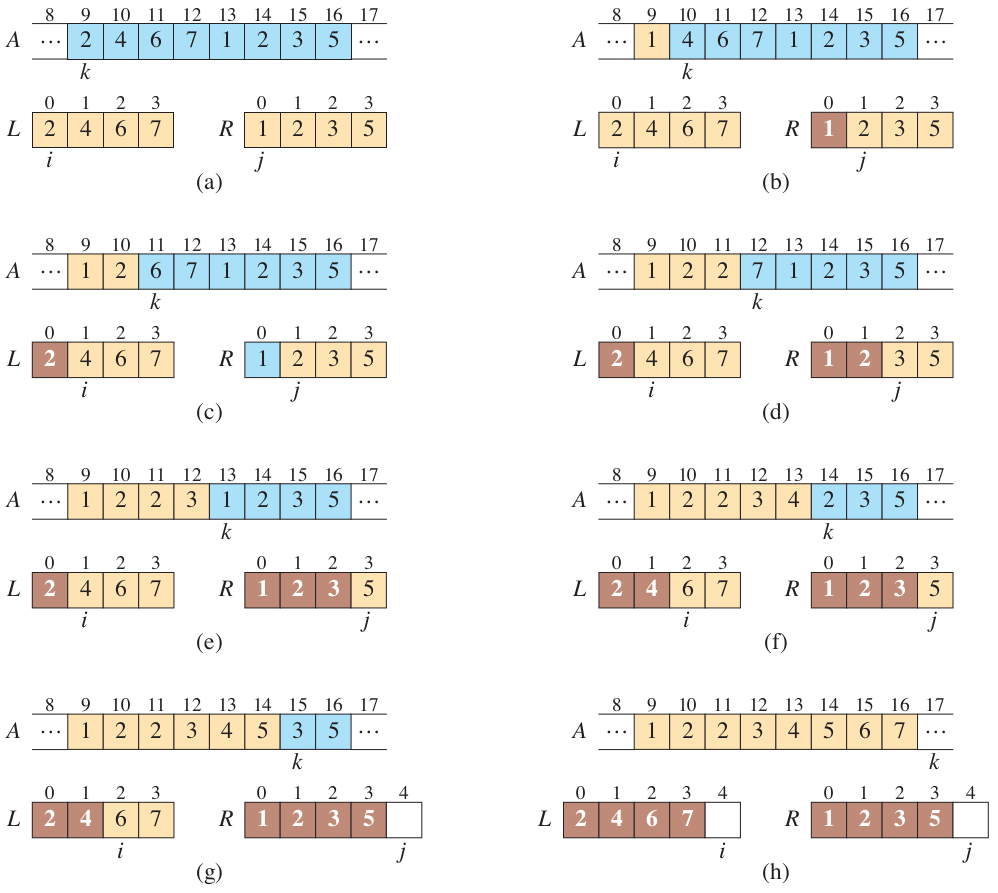
\includegraphics[width=0.5\textwidth]{figs/chap03/merge-example}
\end{figure}
\end{itemize}
\end{frame}


\begin{frame}{‌مرتب‌سازی ادغامی}
\begin{itemize}\itemr
\item[-]
در حلقهٔ تکرار الگوریتم ادغام، در هر تکرار یکی از عناصر در آرایهٔ A کپی می‌شوند و در کل تا پایان الگوریتم n عنصر در آرایه کپی می‌شوند، پس زمان اجرای این الگوریتم
\ath{n}
است.
\end{itemize}
\end{frame}


\begin{frame}{‌مرتب‌سازی ادغامی}
\begin{itemize}\itemr
\item[-]
یک مثال مرتب‌سازی ادغامی در شکل زیر نشان داده شده‌است.
\begin{figure}
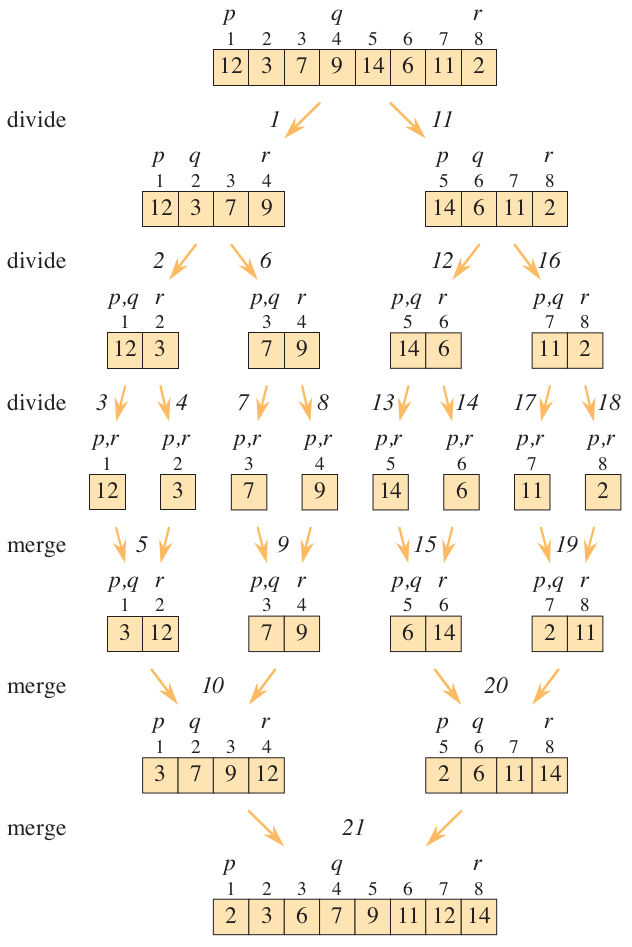
\includegraphics[width=0.3\textwidth]{figs/chap03/merge-sort-example}
\end{figure}
\end{itemize}
\end{frame}


\begin{frame}{‌مرتب‌سازی ادغامی}
\begin{itemize}\itemr
\item[-]
وقتی یک مسئله به صورت بازگشتی طراحی می‌شود، زمان اجرای آن را نیز معمولا با استفاده از معادلات بازگشتی
\fn{1}{recurrence equation}
به دست می‌آوریم.
در این معادلات بازگشتی، زمان اجرای یک الگوریتم با ورودی اندازهٔ n توسط زمان اجرای همان الگوریتم با ورودی‌هایی از اندازه‌های کوچک‌تر به دست می‌آید. روش‌های متعددی برای حل مسائل بازگشتی وجود دارند که می‌توان از آنها استفاده کرد.
\end{itemize}
\end{frame}


\begin{frame}{‌مرتب‌سازی ادغامی}
\begin{itemize}\itemr
\item[-]
به طور کلی اگر فرض کنیم زمان اجرای یک الگوریتم برای ورودی با اندازهٔ n برابر با
\m{T(n)}
باشد و توسط روش تقسیم و حل مسئلهٔ مورد نظر به
\m{a}
زیر مسئله تقسیم شود که اندازه ورودی هر کدام
\m{n/b}
باشد، آنگاه به زمان
\m{aT(n/b)}
برای حل مسئله نیاز داریم.
\item[-]
همچنین اگر به زمان 
\m{D(n)}
 برای تقسیم مسئله به زیر مسئله‌ها و به زمان
\m{C(n)} 
 برای ادغام زیر مسئله‌ها نیاز داشته باشیم، آنگاه این زمان‌ها به زمان مورد نیاز برای حل مسئله افزوده می‌شوند.
\end{itemize}
\end{frame}


\begin{frame}{‌مرتب‌سازی ادغامی}
\begin{itemize}\itemr
\item[-]
فرض کنید در حالت پایه، یعنی وقتی اندازهٔ ورودی از یک مقدار معین کوچکتر است، اجرای برنامه در زمان ثابت انجام شود، یعنی زمان اجرای برنامه در حالت پایه به اندازهٔ ورودی n بستگی نداشته باشد.
\item[-]
در حالت کلی زمان اجرای یک الگوریتم تقسیم و حل را می‌توانیم با استفاده از رابطهٔ بازگشتی زیر بنویسیم.
\begin{align*}
\m{T(n)} = \left\{\begin{array}{lr}
          \m{\Theta (1)}& \m{n < n_0}~\text{اگر}\\
          \m{D(n) + aT(n/b) + C(n)}&\text{در باقی حالات}
\end{array}\right.
\end{align*}
\end{itemize}
\end{frame}


\begin{frame}{‌مرتب‌سازی ادغامی}
\begin{itemize}\itemr
\item[-]
حال زمان اجرای الگوریتم مرتب‌سازی ادغامی را در بدترین حالت به ازای یک آرایهٔ با طول n تحلیل می‌کنیم.\\
۱. تقسیم : تقسیم کردن آرایه به دو قسمت در زمان ثابت انجام می‌شود، بنابراین داریم
\m{D(n) = \ath{1}} .\\
۲. حل : در مرحلهٔ حل از دو آرایه با اندازه
\m{n/2}
به صورت بازگشتی استفاده می‌کنیم بنابراین زمان مورد نیاز در این مرحله برابر است با
\m{2T(n/2)}
. توجه کنید که ممکن است آرایه بر دو بخش پذیر نباشد، اما معمولاً در تحلیل الگوریتم از توابع کف و سقف صرف نظر می‌کنیم، چرا که تأثیری در تحلیل الگوریتم نمی‌گذارند.\\
۳. ترکیب : در این مرحله برای ادغام دو آرایه، جهت تولید یک آرایه با طول n به زمان
\ath{n}
نیاز داریم، بنابراین داریم
\m{C(n) = \ath{n}} .
\end{itemize}
\end{frame}


\begin{frame}{‌مرتب‌سازی ادغامی}
\begin{itemize}\itemr
\item[-]
بنابراین در مجموع زمان اجرای الگوریتم مرتب‌سازی ادغامی به صورت زیر است :
\begin{center}
\m{T(n) = 2T(n/2) + \ath{n}}
\end{center}
\item[-]
با حل این معادله بازگشتی می‌توان به دست آورد
\m{T(n) = \ath{n \lg n}}
، بنابراین زمان مورد نیاز برای اجرای الگوریتم مرتب‌سازی ادغامی از مرتب‌سازی درجی بهتر است.
\end{itemize}
\end{frame}


\begin{frame}{‌مرتب‌سازی ادغامی}
\begin{itemize}\itemr
\item[-]
حال برای اینکه بدون حل معادله بازگشتی، زمان اجرای به دست آمده را درک کنیم، می‌توانیم الگوریتم را به صورت زیر تحلیل کنیم.
\item[-]
برای سادگی فرض می‌کنیم طول آرایهٔ ورودی برابر با n بوده و n توانی از ۲ است. با این ساده‌سازی همیشه با تقسیم n بر ۲ یک عدد صحیح به دست می‌آید.
\item[-]
زمان اجرای الگوریتم را به صورت زیر می‌نویسیم.
\begin{align*}
\m{T(n) =} \left\{\begin{array}{lr}
          \m{c_1} & \m{n = 1}~\text{اگر}\\
          \m{2T(n/2) + c_2n} & \m{n > 1}~ \text{اگر}\\
\end{array}\right.
\end{align*}
\item[-]
در اینجا
\m{c_1}
زمان اجرای الگوریتم است هنگامی که طول ورودی ۱ باشد و
\m{c_2}
مضرب ثابتی است که برای تقسیم و ادغام آرایه با طول n نیاز داریم.
\end{itemize}
\end{frame}


\begin{frame}{‌مرتب‌سازی ادغامی}
\begin{itemize}\itemr
\item[-]
شکل‌های زیر تقسیم این مسئله را به زیر مسئله‌ها و تحلیل زمان زیر مسئله‌ها را نشان می‌دهد.
\LR{
\begin{figure}
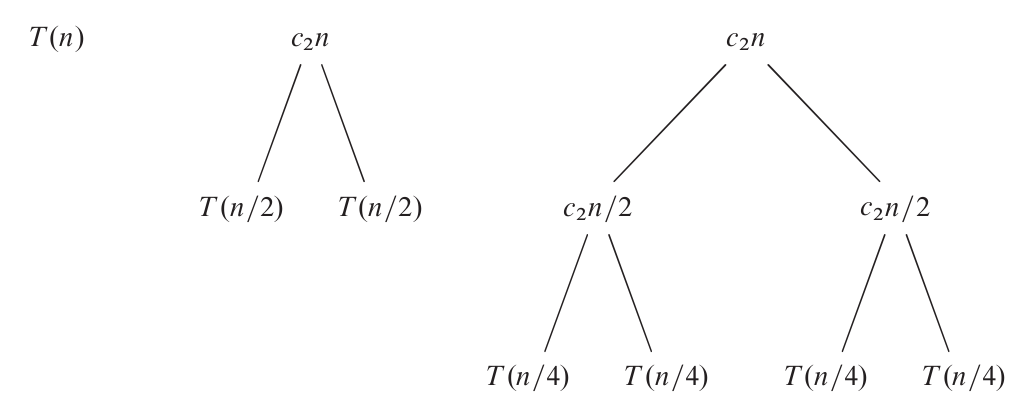
\includegraphics[width=0.5\textwidth]{figs/chap03/merge-sort-analysis1}
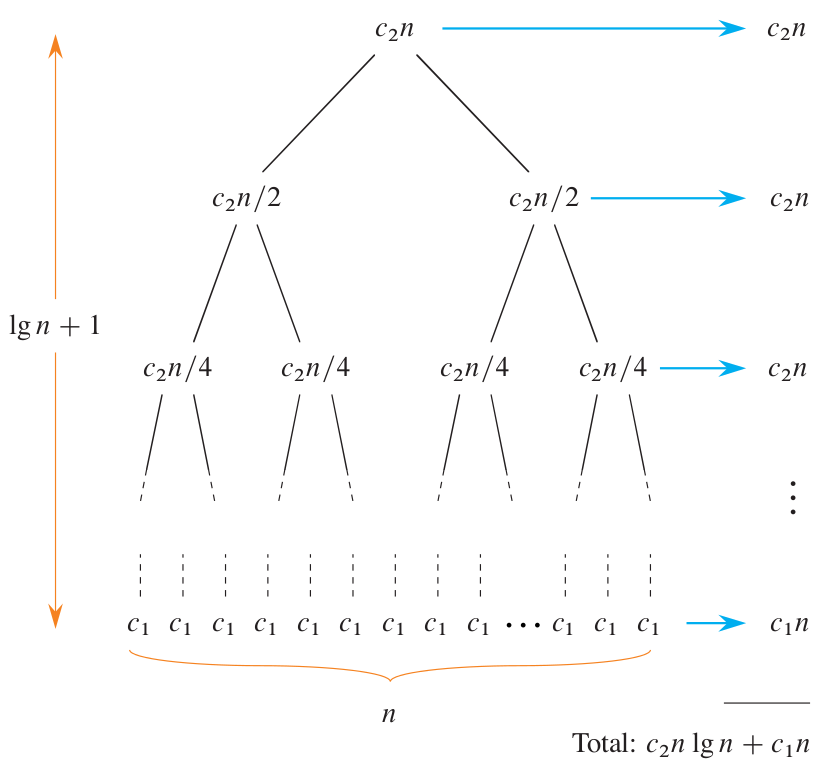
\includegraphics[width=0.4\textwidth]{figs/chap03/merge-sort-analysis2}
\end{figure}
}
\end{itemize}
\end{frame}


\begin{frame}{‌مرتب‌سازی ادغامی}
\begin{itemize}\itemr
\item[-]
مقدار
\m{c_2n}
در ریشهٔ این درخت در واقع زمان مورد نیاز برای تقسیم و ادغام را نشان می‌دهد، هنگامی که اندازهٔ مسئله برابر است با n . دو زیر درخت در سطح ۱ این درخت زمان‌های مورد نیاز را وقتی اندازهٔ ورودی
\m{n/2}
است نشان می‌دهند. هزینه مورد نیاز برای تقسیم و ادغام هر‌کدام از این زیر درخت‌ها برابر است با
\m{c_2n/2}
و مجموعه این هزینه‌ها برای دو زیر درخت برابر است با
\m{c_2n}.
\item[-]
چنانچه این محاسبات را ادامه دهیم، به این نتیجه می‌رسیم که هزینه تقسیم و ادغام برای هر یک از سطوح درخت برابر است با
\m{c_2n}.
\end{itemize}
\end{frame}


\begin{frame}{‌مرتب‌سازی ادغامی}
\begin{itemize}\itemr
\item[-]
سطح آخر، یعنی سطحی که برگ‌های درخت در آن قرار دارد، حالت پایه را نشان می‌دهد که در این حالت زمان اجرای هر یک از زیر آرایه‌ها برابر است با
\m{c_1}
و چون تعداد n زیر آرایه با طول ۱ داریم، زمان اجرا برای کل زیر آرایه‌ها برابر است با
\m{c_1 n}.
\item[-]
از آنجایی که این درخت در هر مرحله به دو بخش تقسیم می‌شود، تعداد سطوح درخت برابر است با
\m{\lg n + 1}.
\item[-]
بنابراین زمان کل اجرای الگوریتم برابر است با
\m{c_2n \lg n+ c_1n} .
\item[-]
می‌توانیم با استفاده از تحلیل مجانبی بنویسیم
\m{T(n) = \ath{n \lg n}}.
\end{itemize}
\end{frame}


\begin{frame}{‌جستجوی دودویی}
\begin{itemize}\itemr
\item[-]
برای جستجوی یک مقدار در یک آرایه باید همهٔ عناصر آرایه را یک‌به‌یک بررسی کنیم. این جستجو برای یک آرایه با
\m{n}
عنصر در زمان
\m{O(n)}
انجام می‌شود.
\item[-]
حال فرض می‌کنیم می‌خواهیم یک مقدار را در یک آرایه مرتب شده پیدا کنیم.
\item[-]
برای این کار می‌توانیم از یک الگوریتم تقسیم و حل به نام جستجوی دودویی
\fn{1}{binary search}
استفاده کنیم.
\end{itemize}
\end{frame}


\begin{frame}{‌جستجوی دودویی}
\begin{itemize}\itemr
\item[-]
الگوریتم تقسیم و حل آرایه را به دو قسمت تقسیم می‌کند. برای جستجوی مقدار
\code{x}
در آرایه
\code{A}
، ابتدا مقدار
\code{x}
با عنصر وسط آرایه یعنی
\code{A[n/2]}
مقایسه می‌شود. اگر
\code{x}
برابر با مقدار وسط آرایه بود، مقدار مورد نظر یافته شده است. اگر
\code{x}
کوچکتر از عنصر وسط آرایه بود، باید
\code{x}
را در نیمه اول آرایه یعنی\\
\code{A[1:n/2-1]}
جستجو کنیم. در غیراینصورت باید
\code{x}
را در نیمه دوم آرایه یعنی
\code{A[n/2+1:n]}
جستجو کنیم. این روند را برای زیر آرایه‌ها ادامه می‌دهیم تا یا
\code{x}
یافته شود یا مشخص شود که
\code{x}
در آرایه وجود ندارد.
\end{itemize}
\end{frame}


\begin{frame}{‌جستجوی دودویی}
\begin{itemize}\itemr
\item[-]
بنابراین مراحل انجام جستجوی دودویی به صورت زیر است.
\item[۱.]
تقسیم : برای پیدا کردن مقدار
\code{x}
در آرایه
\code{A[low:high]}
قرار می‌دهیم
\code{mid=$\lfloor$(low + high)/2$\rfloor$} .
اگر
\code{A[mid]}
برابر با
\code{x}
بود به نتیجه رسیده‌ایم در غیراینصورت آرایه را به دو قسمت
\code{A[low:mid-1]}
و
\code{A[mid+1:high]}
تقسیم می‌کنیم. این تقسیم تنها در صورتی می‌تواند انجام شود که
\code{high}
از
\code{low}
بزرگ‌تر باشد.
\item[۲.]
حل : در صورتی که مقدار
\code{x}
از
\code{A[mid]}
کوچکتر بود، الگوریتم جستجو برای
\code{A[low:mid-1]}
فراخوانی می‌شود، در غیراینصورت برای
\code{A[mid+1:high]}
فراخوانی می‌شود.
\item[۳.]
ترکیب : در گام ترکیب هیچ عملیاتی انجام نمی‌شود.
\end{itemize}
\end{frame}


\begin{frame}{‌جستجوی دودویی}
\begin{itemize}\itemr
\item[-]
برای پیدا کردن عدد ۱۸ در آرایهٔ زیر، الگوریتم به صورت زیر عمل می‌کند.
\begin{figure}
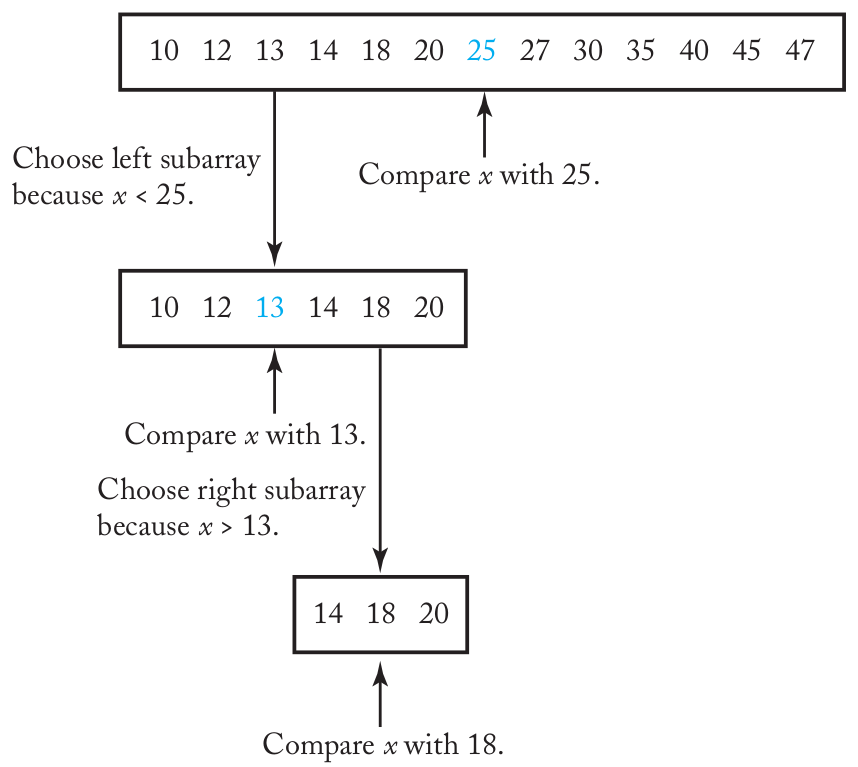
\includegraphics[width=0.55\textwidth]{figs/chap03/binarysearch2-1}
\end{figure}
\end{itemize}
\end{frame}


\begin{frame}{‌جستجوی دودویی}
\begin{itemize}\itemr
\item[-]
الگوریتم جستجوی دودویی به صورت زیر است.
\begin{algorithm}[H]\alglr
  \caption{‌Binary Search} 
  \begin{algorithmic}[1]
   \Func{BinarySearch}{A, x, low, high}
   \If{(low > high)}
        \State \Return -‌1
    \EndIf
    \State mid = $\lfloor$(low + high)/2$\rfloor$
    \If{(x == A[mid])}
         \State \Return mid
     \EndIf
     \If{(x < A[mid])}
          \State \Return BinarySearch (A, x, low, mid-1)
      \Else
          \State \Return BinarySearch (A, x, mid+1, high)
      \EndIf                          
  \end{algorithmic}
  \label{alg:merge}
\end{algorithm}
\item[-]
برای جستجوی مقدار
\code{x}
جستجوی دودویی باید به صورت
\code{BinarySearch(A, x, 1, n)}
فراخوانی شود.
\end{itemize}
\end{frame}



\begin{frame}{‌جستجوی دودویی}
\begin{itemize}\itemr
\item[-]
در تقسیم یک آرایه به دو قسمت صرفا یک عملیات تقسیم انجام می‌شود. بنابراین
\m{D(n) = O(1)}
. تقسیم آرایه در زمان ثابت انجام می‌شود.
\item[-]
بنابراین زمان اجرای الگوریتم جستجوی دودویی برای آرایه با
\m{n}
عنصر برابر است با زمان اجرای الگوریتم برای آرایه‌ای با
\m{n/2}
عنصر به علاوه یک زمان ثابت.
\item[-]
می‌توانیم بنویسیم
\m{T(n) = T(\frac{n}{2}) + O(1)}
و
\m{T(1) = 1}
\item[-]
با حل این رابطه بازگشتی به دست می‌آوریم
\m{T(n) = O(\lg n)}.
\end{itemize}
\end{frame}


\begin{frame}{‌مرتب‌سازی سریع}
\begin{itemize}\itemr
\item[-]
یکی از الگوریتم‌های مرتب‌سازی بسیار پر استفاده الگوریتم مرتب‌سازی سریع
\fn{1}{quicksort algorithm}
است.
\item[-]
این الگوریتم یک الگوریتم تقسیم و حل است. زمان اجرای آن در بدترین حالت
\ath{n^2}
است، اما در حالت میانگین در زمان
\ath{n \lg n}
اجرا می‌شود. این الگوریتم به حافظه اضافی نیاز ندارد.
\end{itemize}
\end{frame}


\begin{frame}{‌مرتب‌سازی سریع}
\begin{itemize}\itemr
\item[-]
برای مرتب‌سازی آرایه
\code{A[p:r]}
این الگوریتم از روش تقسیم و حل به صورت زیر استفاده می‌کند.
\item[۱.]
تقسیم : آرایهٔ
\code{A[p:r]}
به دو قسمت
\code{A[p:q-1]}
(قسمت پایین)
\fn{1}{low side}
و
\code{A[q+1:r]}
(قسمت بالا)
\fn{2}{high side}
تقسیم می‌شود به طوری که همه عناصر قسمت پایین از عنصر
\code{A[q]}
(عنصر محور)
\fn{3}{pivot}
کوچکتر یا برابرند و عناصر قسمت بالا از عنصر محور بزرگ‌ترند.
\item[۲.]
حل : الگوریتم مرتب‌سازی سریع برای دو زیر آرایه
\code{A[p:q-1]}
و
\code{A[q+1:r]}
فراخوانی می‌شود.
\item[۳.]
ترکیب : در این قسمت هیچ عملیاتی انجام نمی‌شود. از آنجایی که همه عناصر
\code{A[p:q-1]}
مرتب شده و کوچکتر یا مساوی
\code{A[q]}
هستند و همهٔ عناصر
\code{A[q+1:r]}
مرتب شده و بزرگتر از
\code{A[q]}
هستند، بنابراین کل آرایه
\code{A[p:r]}
مرتب شده است.
\end{itemize}
\end{frame}

\begin{frame}{‌مرتب‌سازی سریع}
\begin{itemize}\itemr
\item[-]
در تقسیم آرایه به دو قسمت پایین و بالا، فرض کنید قسمت کرمی رنگ در شکل زیر عناصری باشند که مقدار آنها از عنصر محوری x کمتر و قسمت آبی رنگ عناصری باشند که مقدار آنها از عنصر محوری بیشتر است.
\begin{figure}
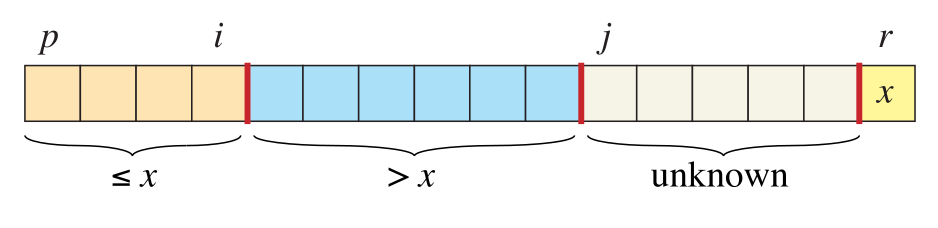
\includegraphics[width=0.7\textwidth]{figs/chap03/quicksort1}
\end{figure}
\end{itemize}
\end{frame}


\begin{frame}{‌مرتب‌سازی سریع}
\begin{itemize}\itemr
\item[-]
اندیس i مرز بین قسمت پایین و قسمت بالا را نگهداری می‌کند. توسط اندیس j عناصر آرایه یک به یک بررسی می‌شوند. در صورتی که مقدار آنها از عنصر محوری x کمتر باشد به صورت زیر به قسمت پایین منتقل می‌شوند و مرز قسمت پایین و بالا تغییر می‌کند، در غیر اینصورت قسمت در مکان خود نگه داشته می‌شوند.
\begin{figure}
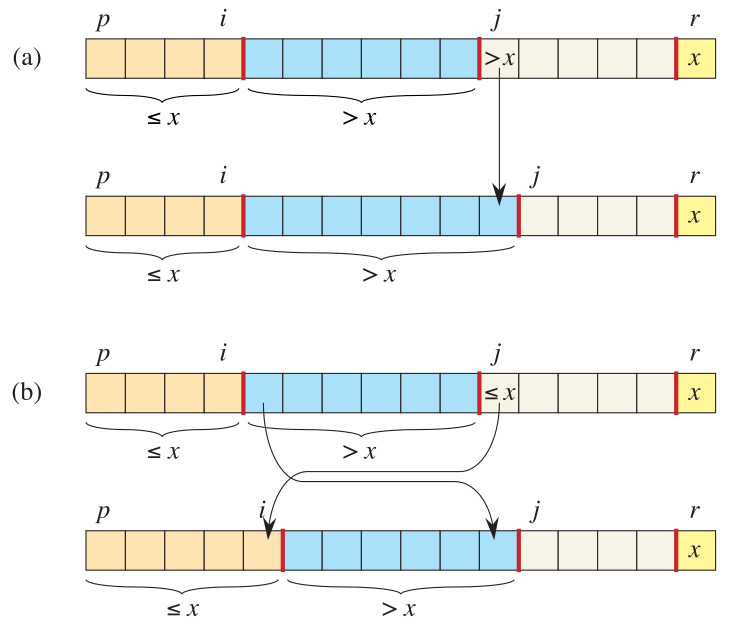
\includegraphics[width=0.5\textwidth]{figs/chap03/quicksort2}
\end{figure}
\end{itemize}
\end{frame}


\begin{frame}{‌مرتب‌سازی سریع}
\begin{itemize}\itemr
\item[-]
در شکل زیر نحوه اجرای الگوریتم تقسیم‌بندی نشان داده شده است. عنصر محور در اینجا برابر است با
\code{A[r]}.
\begin{figure}
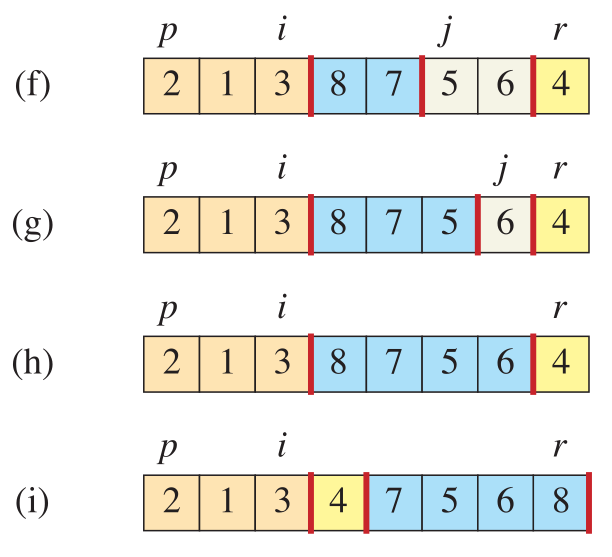
\includegraphics[width=0.4\textwidth]{figs/chap03/partition2}
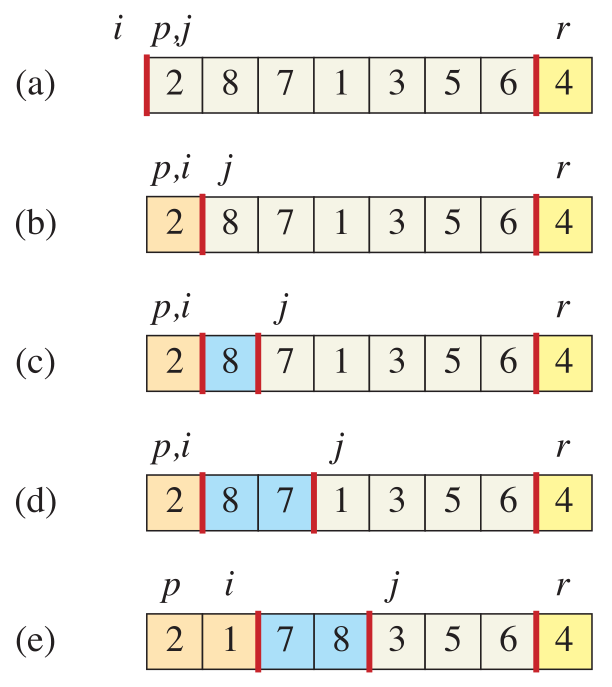
\includegraphics[width=0.4\textwidth]{figs/chap03/partition1}
\end{figure}
\end{itemize}
\end{frame}



\begin{frame}{‌مرتب‌سازی سریع}
\begin{itemize}\itemr
\item[-]
الگوریتم مرتب‌سازی سریع به صورت زیر است.
\begin{algorithm}[H]\alglr
  \caption{Quicksort} 
  \begin{algorithmic}[1]
   \Func{Quicksort}{A, p, r}
   \If{p < r}
           \LeftComment{Partition the subarray around the pivot, which ends up in A[q].}
           \State q = Partition (A, p, r)
           \State Quicksort (A, p, q-1) \LeftComment{recursively sort the low side}
           \State Quicksort (A, q+1, r) \LeftComment{recursively sort the high side}
    \EndIf                           
  \end{algorithmic}
  \label{alg:merge}
\end{algorithm}
\end{itemize}
\end{frame}


\begin{frame}{‌مرتب‌سازی سریع}
\begin{itemize}\itemr
\item[-]
الگوریتم تقسیم‌بندی
\fn{1}{partition}
باید عناصر آرایه را به گونه‌ای جابجا کند که همهٔ عناصر قسمت پایین از عنصر محور کوچک‌تر یا مساوی و عناصر قسمت بالا از عنصر محور بزرگ‌تر باشند.
\end{itemize}
\end{frame}


\begin{frame}{‌مرتب‌سازی سریع}
\begin{itemize}\itemr
\item[-]
الگوریتم تقسیم بندی به صورت زیر است.
\begin{algorithm}[H]\alglr
  \caption{Partition} 
  \begin{algorithmic}[1]
   \Func{Partition}{A, p, r}
   \State x = A[r] \LeftComment{the pivot}
   \State i = p - 1 \LeftComment{highest index into the low side}
   \For{j = p \To r-1} \LeftComment{process each element other than the pivot}
        \If{A[j] <= x} \LeftComment{does this element belong on the low side?}
            \State i = i+1 \LeftComment{index of a new slot in the low side}
            \State exchange A[i] with A[j] \LeftComment{put this element there}
        \EndIf
   \EndFor 
   \State exchange A[i+1] with A[r] \LeftComment{pivot goes just to the right of the low side}
   \State \Return i+1 \LeftComment{new index of the pivot}
  \end{algorithmic}
  \label{alg:merge}
\end{algorithm}
\end{itemize}
\end{frame}


\begin{frame}{‌مرتب‌سازی سریع}
\begin{itemize}\itemr
\item[-]
زمان اجرای الگوریتم مرتب‌سازی سریع به نحوه تقسیم‌بندی آرایه بستگی دارد. اگر تقسیم‌بندی آرایه متوازن نباشد الگوریتم در زمان
\ath{n^2}
اجرا می‌شود اما اگر تقسیم‌بندی متوازن باشد، الگوریتم در زمان
\ath{n \lg n}
اجرا می‌شود.
\end{itemize}
\end{frame}


\begin{frame}{‌مرتب‌سازی سریع}
\begin{itemize}\itemr
\item[-]
اگر در هر بار تقسیم‌بندی آرایه، یک قسمت
\m{n-1}
عنصر و قسمت دیگر
\m{0}
عنصر داشته باشد، آنگاه تقسیم‌بندی نامتوازن است. هزینه تقسیم‌بندی آرایه برابراست با
\ath{n}
. مرتب‌سازی یک آرایه با صفر عنصر در زمان ثابت انجام می‌شود یعنی
\m{T(0) = \ath{1}}
بنابراین خواهیم داشت :
\begin{align*}
\m{T(n) = T(n-1) + T(0) + \ath{n} = T(n-1) + \ath{n}}
\end{align*}
\item[-]
با حل کردن این رابطه بازگشتی به دست می‌آوریم
\m{T(n) = \ath{n^2}}.
\item[-]
بنابراین در بدترین حالت الگوریتم مرتب‌سازی سریع مانند مرتب‌سازی درجی عمل می‌کند. بدترین حالت در مرتب‌سازی سریع وقتی رخ می‌دهد که آرایه کاملا مرتب باشد.
\end{itemize}
\end{frame}


\begin{frame}{‌مرتب‌سازی سریع}
\begin{itemize}\itemr
\item[-]
اگر الگوریتم تقسیم‌بندی، آرایه را به دو قسمت مساوی تقسیم کند، آنگاه می‌توانیم زمان اجرای الگوریتم را با استفاده از رابطه بازگشتی زیر محاسبه کنیم.
\begin{align*}
\m{T(n) = 2 T(n/2) + \ath{n}}
\end{align*}
\item[-]
با حل این رابطه به دست می‌آوریم
\m{T(n) = \ath{n \lg n}}.
\item[-]
می‌توان اثبات کرد که الگوریتم مرتب‌سازی سریع در حالت میانگین در زمان
\ath{n \lg n}
اجرا می‌شود.
حالت میانگین وقتی است که در الگوریتم تقسیم‌بندی، آرایه به طور میانگین با یک نسبت معین به دو قسمت تقسیم شود.
\end{itemize}
\end{frame}



\begin{frame}{‌مرتب‌سازی سریع}
\begin{itemize}\itemr
\item[-]
همچنین برای اینکه بدترین حالت اتفاق نیافتد، می‌توان عنصر محوری را به صورت تصادفی انتخاب کرد و اثبات کرد که در این صورت زمان اجرای الگوریتم مرتب‌سازی سریع
\ath{n \lg n}
خواهد بود.
\item[-]
یک روش دیگر برای اینکه بدترین حالت اتفاق نیافتد این است که بین اولین عنصر، آخرین عنصر، و عنصر وسط از آرایه، عنصری که مقدار آن میانهٔ دو مقدار دیگر است را به عنوان عنصر محوری انتخاب کنیم. این روش به استراتژی انتخاب میانهٔ سه مقدار 
\fn{1}{median of three values}
معروف است.
\end{itemize}
\end{frame}

\begin{frame}{‌ضرب ماتریس‌ها}
\begin{itemize}\itemr
\item[-]
از روش تقسیم و حل می‌توانیم برای ضرب ماتریس‌های مربعی استفاده کنیم.
\item[-]
فرض کنید
\m{A = (a_{ij})}
و
\m{B = (b_{ij})}
دو ماتریس
\m{n \times n}
باشند. ماتریس
\m{C = A \cdot B}
نیز یک ماتریس
\m{n \times n}
است که درایه‌های آن به صورت زیر محاسبه می‌شوند.
\begin{flushleft}
\m{c_{ij} = \sum_{k=1}^{n} a_{ik} \cdot b_{kj}}
\end{flushleft}
\end{itemize}
\end{frame}


\begin{frame}{‌ضرب ماتریس‌ها}
\begin{itemize}\itemr
\item[-]
الگوریتم ضرب دو ماتریس در زیر نوشته شده‌است.
\begin{algorithm}[H]\alglr
  \caption{Matrix} 
  \begin{algorithmic}[1]
    \Func{Matrix-Multiply}{A, B, C, n}
       \For{i = 1 \To n} \LeftComment{compute entries in each of n rows}
           \For{j = 1 \To n} \LeftComment{compute n entries in row i}
			   \For{k = 1 \To n}
					\State c[i,j] = c[i,j] + a[i,k] * b[k,j] \LeftComment{compute c[i,j]}
			    \EndFor
			\EndFor
	   \EndFor 
     \end{algorithmic}
  \label{alg:merge}
\end{algorithm}
\item[-]
از آنجایی که خط ۴ باید
\m{n^3}
بار تکرار شود، بنابراین زمان مورد نیاز برای اجرای این الگوریتم برابر است با
\ath{n^3}.
\end{itemize}
\end{frame}

\begin{frame}{‌ضرب ماتریس‌ها}
\begin{itemize}\itemr
\item[-]
حال می‌خواهیم ضرب دو ماتریس را توسط روش تقسیم و حل محاسبه کنیم.
\item[-]
در مرحله تقسیم، یک ماتریس
\m{n \times n}
را به چهار ماتریس
\m{n/2 \times n/2}
تقسیم می‌کنیم. برای سادگی فرض می‌کنیم n توانی از ۲ باشد و امکان تقسیم کردن آن به ۲ در فرایند الگوریتم تقسیم و حل وجود داشته باشد.
\end{itemize}
\end{frame}


\begin{frame}{‌ضرب ماتریس‌ها}
\begin{itemize}\itemr
\item[-]
با فرض اینکه هر یک از ماتریس‌های
A
,
B
و
C
را به چهار قسمت تقسیم کنیم، محاسبات به صورت زیر انجام می‌شود.
\begin{align*}
\m{C = A \cdot B \Rightarrow} \left( \begin{array}{cc} \m{C_{11}} & \m{C_{12}} \\ \m{C_{21}} & \m{C_{22}} \end{array} \right)
= \left( \begin{array}{cc} \m{A_{11}} & \m{A_{12}} \\ \m{A_{21}} & \m{A_{22}} \end{array} \right)
\left( \begin{array}{cc} \m{B_{11}} & \m{B_{12}} \\ \m{B_{21}} & \m{B_{22}} \end{array} \right)
\end{align*}
\item[-]
بنابراین خواهیم داشت :
\begin{align*}
\m{C_{11} = A_{11} \cdot B_{11} + A_{12} \cdot B_{21}}\\
\m{C_{12}= A_{11} \cdot B_{12} + A_{12} \cdot B_{22}}\\
\m{C_{21}= A_{21} \cdot B_{11} + A_{22} \cdot B_{21}}\\
\m{C_{22}= A_{21} \cdot B_{12} + A_{22} \cdot B_{22}}
\end{align*}
\end{itemize}
\end{frame}



\begin{frame}{‌ضرب ماتریس‌ها}
\begin{itemize}\itemr
\item[-]
بنابراین ضرب یک جفت ماتریس 
\m{n \times n}
را به ضرب هشت جفت ماتریس 
\m{n/2 \times n/2}
تبدیل کردیم.
\item[-]
توجه کنید که در این محاسبات نتیجهٔ ضرب
\m{A_{11} \cdot B_{11}}
و همچنین
\m{A_{12} \cdot B_{21}}
باید در 
\m{C_{11}}
ذخیره شود.
\begin{align*}
\m{C_{11} = A_{11} \cdot B_{11} + A_{12} \cdot B_{21}}\\
\m{C_{12}= A_{11} \cdot B_{12} + A_{12} \cdot B_{22}}\\
\m{C_{21}= A_{21} \cdot B_{11} + A_{22} \cdot B_{21}}\\
\m{C_{22}= A_{21} \cdot B_{12} + A_{22} \cdot B_{22}}
\end{align*}
\item[-]
حالت پایه در این الگوریتم وقتی است که می خواهیم دو ماتریس
\m{1 \times 1}
را در هم ضرب کنیم که در این حالت در واقع دو عدد را در هم ضرب می‌کنیم.
\end{itemize}
\end{frame}


\begin{frame}{‌ضرب ماتریس‌ها}
\begin{itemize}\itemr
\item[-]
الگوریتم تقسیم و حل برای ضرب دو ماتریس را می‌توانیم به صورت زیر بنویسیم.
\begin{algorithm}[H]\alglr
  \caption{Matrix} 
  \begin{algorithmic}[1]
    \Func{Matrix-Multiply-Recursive}{A, B, C, n}
   \Statex \LeftComment{Base case.}    
    \If{n==1}
    	\State \mc{c_{11}} = \mc{c_{11}} + \mc{a_{11}} * \mc{b_{11}}
    	\State \Return
    \EndIf
   \Statex \LeftComment{Divide.}
   \State Partition A, B, and C into n/2 \mc{\times} n/2 submatrices 
    	\Statex \mc{A_{11}, A_{12}, A_{21}, A_{22}}; 
    	\Statex \mc{B_{11}, B_{12}, B_{21}, B_{22}};
    	\Statex \mc{C_{11}, C_{12}, C_{21}, C_{22}}; respectively    
  \end{algorithmic}
  \label{alg:merge}
\end{algorithm}
\end{itemize}
\end{frame}


\begin{frame}{‌ضرب ماتریس‌ها}
\begin{itemize}\itemr
\item[-]
\begin{algorithm}[H]\alglr
  \caption{Matrix} 
  \begin{algorithmic}[1]
    \setcounter{ALG@line}{4}
   \Statex \LeftComment{Conquer.}   
    	\State Matrix-Multiply-Recursive (\mc{A_{11}, B_{11}, C_{11}, n/2})
    	\State Matrix-Multiply-Recursive (\mc{A_{11}, B_{12}, C_{12}, n/2})
    	\State Matrix-Multiply-Recursive (\mc{A_{21}, B_{11}, C_{21}, n/2})
    	\State Matrix-Multiply-Recursive (\mc{A_{21}, B_{12}, C_{22}, n/2})
    	\State Matrix-Multiply-Recursive (\mc{A_{12}, B_{21}, C_{11}, n/2})
    	\State Matrix-Multiply-Recursive (\mc{A_{12}, B_{22}, C_{12}, n/2})
    	\State Matrix-Multiply-Recursive (\mc{A_{22}, B_{21}, C_{21}, n/2})
    	\State Matrix-Multiply-Recursive (\mc{A_{22}, B_{22}, C_{22}, n/2})
  \end{algorithmic}
  \label{alg:merge}
\end{algorithm}
\end{itemize}
\end{frame}


\begin{frame}{‌ضرب ماتریس‌ها}
\begin{itemize}\itemr
\item[-]
یک ضرب ماتریسی با اندازهٔ 
\m{n}
 را به ۸ ضرب ماتریسی با اندازهٔ 
\m{n/2}
تبدیل کردیم.
\item[-]
فرض می‌کنیم که در تقسیم ماتریس به ماتریس‌های کوچک‌تر، تنها اندیس‌ها را نامگذاری مجدد می‌کنیم و بنابراین عملیات در زمان ثابت می‌تواند انجام شود.
\item[-]
بنابراین برای تحلیل این الگوریتم، می‌توانیم از رابطه بازگشتی زیر استفاده کنیم.
\begin{center}
\m{T(n) = 8 T(n/2) +  \ath{1}}
\end{center}
\end{itemize}
\end{frame}


\begin{frame}{‌ضرب ماتریس‌ها}
\begin{itemize}\itemr
\item[-]
با حل کردن این معادله به دست می‌آوریم
\m{T(n) = \ath{n^3}}.
\item[-]
بنابراین روش تقسیم و حل زمان محاسبات را در ضرب ماتریسی کاهش نمی‌دهد.
\item[-]
با استفاده از الگوریتم استراسن
\fn{1}{Strassen}
که از یک الگوریتم تقسیم و حل بهینه‌تر استفاده می‌کند، زمان محاسبات کاهش پیدا خواهد کرد.
\end{itemize}
\end{frame}

\begin{frame}{‌الگوریتم استراسن}
\begin{itemize}\itemr
\item[-]
ضرب دو ماتریس
\m{n \times n}
را در زمان کمتر از
\m{n^3}
نیز می‌توان انجام داد. از آنجایی که برای ضرب دو ماتریس مربعی با اندازهٔ n دقیقا به
\m{n^3}
گام محاسباتی نیاز است،‌ بسیاری بر این باور بودند که ضرب ماتریسی نمی‌تواند در زمانی کمتر صورت بگیرد تا اینکه در سال ۱۹۶۹ ولکر استراسن
\fn{1}{Volker Strassen}
 ریاضیدان آلمانی، الگوریتمی با زمان اجرای
\ath{n^{\lg 7}}
ابداع کرد. از آنجایی که
\m{\lg 7 = 2.8073 ...}
، بنابراین می‌توان گفت الگوریتم استراسن در زمان
\abo{n^{2.81}}
ضرب دو ماتریس را محاسبه می‌کند.
\item[-]
الگوریتم استراسن یک الگوریتم از نوع و تقسیم و حل است.
\item[-]
استراسن مجددا در سال ۱۹۸۶ الگوریتمی از مرتبه
\abo{n^{2.48}}
ارائه داد.
در سال ۱۹۹۰ الگوریتمی از مرتبه
\abo{n^{2.38}}
و در سال ۲۰۲۳ یک الگوریتم بهبود یافته ارائه شد.
 جستجو برای پیدا کردن سریع‌ترین الگوریتم ضرب ماتریسی همچنان ادامه دارد.
\end{itemize}
\end{frame}


\begin{frame}{‌الگوریتم استراسن}
\begin{itemize}\itemr
\item[-]
ایدهٔ الگوریتم استراسن این است که در مراحل تقسیم و ترکیب از عملیات بیشتری استفاده می‌کند و بنابراین مراحل تقسیم و ترکیب در این الگوریتم نسبت به مراحل تقسیم و ترکیب در الگوریتم تقسیم و حل عادی زمان بیشتری صرف می‌کند ولی در ازای این افزایش زمان، در مرحله حل بازگشتی زمان کمتری مصرف می‌شود. در واقع در مرحله بازگشتی به جای فراخوانی ۸ تابع بازگشتی ۷ تابع بازگشتی فراخوانی می‌شوند.
\item[-]
به عبارت دیگر عملیات مورد نیاز برای یکی از فراخوانی‌های بازگشتی توسط تعدادی عملیات جمع در مراحل تقسیم و ترکیب انجام می‌شود.
\end{itemize}
\end{frame}


\begin{frame}{‌الگوریتم استراسن}
\begin{itemize}\itemr
\item[-]
به عنوان مثال فرض کنید می‌خواهیم به ازای دو عدد دلخواه 
\m{x}
 و 
\m{y}
  ، مقدار
\m{x^2 - y^2}
را محاسبه کنیم. اگر بخواهیم این محاسبات را به صورت معمولی انجام دهیم، باید ابتدا x و y را به توان ۲ برسانیم و سپس دو مقدار به دست آمده را از هم کم کنیم. اما یک روش دیگر برای این محاسبات وجود دارد.
\item[-]
می‌دانیم
\m{x^2 - y^2 = (x+y)(x-y)}
، بنابراین می‌توانیم این محاسبات را با یک عمل ضرب و دو عمل جمع و تفریق انجام دهبم. اگر x و y دو عدد باشند،‌ زمان انجام محاسبات تفاوت چندانی نخواهد کرد، اما اگر x و y دو ماتریس بزرگ باشند، یک عمل ضرب کمتر بهبود زیادی در زمان اجرا ایجاد می‌کند.
\item[-]
توجه کنید که جمع دو ماتریس مربعی با اندازهٔ n در زمان 
\m{O(n^2)}
انجام می‌شود، و ضرب دو ماتریس در زمان
\m{O(n^3)} .
\end{itemize}
\end{frame}


\begin{frame}{‌الگوریتم استراسن}
\begin{itemize}\itemr
\item[-]
حال که با ایدهٔ الگوریتم استراسن آشنا شدیم، الگوریتم را بررسی می‌کنیم.\\
۱. اگر
\m{n=1}
، آنگاه هر ماتریس تنها یک درایه دارد. در این صورت باید یک عملیات ضرب ساده انجام داد که در زمان
\ath{1}
امکان پذیر است. اگر
\m{n \neq 1}
، آنگاه هر یک از ماتریس‌های ورودی
\m{A}
و
\m{B}
 را به چهار ماتریس
\m{n/2 \times n/2}
تقسیم می‌کنیم. این عملیات نیز در
\ath{1}
امکان پذیر است.\\
۲. با استفاده از زیر ماتریس‌های به دست آمده از مرحله قبل تعداد ۱۰ ماتریس
\m{S_1, S_2, ..., S_{10}}
محاسبه می‌شوند. این عملیات در زمان
\ath{n^2}
انجام می‌شود.\\
۳. تابع ضرب ماتریسی به تعداد ۷ بار بر روی ماتریس‌های
\m{S_i}, \m{A_{ij}}, \m{B_{ij}}
که ابعاد هر کدام 
\m{n/2 \times n/2}
است، به طور بازگشتی انجام می‌شود. نتیجهٔ این محاسبات در ۷ ماتریس
\m{P_1, P_2, ..., P_7}
ذخیره می‌شود.
عملیات این مرحله در زمان
\m{7 T(n/2)}
انجام می‌شود.\\
۴. با استفاده از ماتریس‌های
\m{P_1, P_2, ..., P_7}
، ماتریس‌های
\m{C_{11}, C_{12}, C_{21}, C_{22}}
محاسبه می‌شود. این عملیات نیز در زمان
\ath{n^2}
انجام می‌شود.
\end{itemize}
\end{frame}


\begin{frame}{‌الگوریتم استراسن}
\begin{itemize}\itemr
\item[-]
بنابراین  زمان کل مورد نیاز برای الگوریتم استراسن از رابطه بازگشتی زیر به دست می‌آید.
\begin{flushleft}
\m{T(n) = 7 T(n/2) + \ath{n^2}}
\end{flushleft}
\item[-]
با حل این رابطه بازگشتی به دست می‌آوریم :
\begin{flushleft}
\m{T(n) = \ath{n^{\lg 7}} = O(n^{2.81})}
\end{flushleft}
\end{itemize}
\end{frame}


\begin{frame}{‌الگوریتم استراسن}
\begin{itemize}\itemr
\item[-]
حال ببینیم ماتریس‌های
\m{P_k}
چگونه با استفاده از ماتریس‌های
\m{A_{ij}}
و
\m{B_{ij}}
محاسبه می‌شوند.
\end{itemize}
\end{frame}


\begin{frame}{‌الگوریتم استراسن}
\begin{itemize}\itemr
\item[-]
در مرحلهٔ اول تعداد ۱۰ ماتریس 
\m{S_i}
 به صورت زیر محاسبه می‌شوند.
\begin{align*}
&\m{S_1 = B_{12} - B_{22}}\\
&\m{S_2 = A_{11} + A_{12}}\\
&\m{S_3 = A_{21} + A_{22}}\\
&\m{S_4 = B_{21} - B_{11}}\\
&\m{S_5 = A_{11} + A_{22}}\\
&\m{S_6 = B_{11} + B_{22}}\\
&\m{S_7 = A_{12} - A_{22}}\\
&\m{S_8 = B_{21} + B_{22}}\\
&\m{S_9 = A_{11} - A_{21}}\\
&\m{S_{10} = B_{11} + B_{12}}\\
\end{align*}
\end{itemize}
\end{frame}


\begin{frame}{‌الگوریتم استراسن}
\begin{itemize}\itemr
\item[-]
در محاسبات فوق ۱۰ بار ماتریس‌های
\m{n/2 \times n/2}
را با هم جمع کردیم که این عملیات در زمان
\ath{n^2}
امکان پذیر است.
\end{itemize}
\end{frame}


\begin{frame}{‌الگوریتم استراسن}
\begin{itemize}\itemr
\item[-]
در مرحلهٔ بعد ۷ ماتریس 
\m{P_i}
 را با استفاده از زیر ماتریس‌های 
\m{A_{ij}}
  و 
\m{B_{ij}}
   و ماتریس‌های 
\m{S_i}
    بدست می‌آوریم.
\begin{align*}
&\m{P_1 = A_{11} \cdot S_1 (= A_{11} \cdot B_{12} - A_{11} \cdot B_{22})}\\
&\m{P_2 = S_2 \cdot B_{22} (= A_{11} \cdot B_{22} + A_{12} \cdot B_{22})} \\
&\m{P_3 = S_3 \cdot B_{11} (= A_{21} \cdot B_{11} + A_{22} \cdot B_{11})}\\
&\m{P_4 = A_{22} \cdot S_4 (= A_{22} \cdot B_{21} - A_{22} \cdot B_{11})}\\
&\m{P_5 = S_5 \cdot S_6 (= A_{11} \cdot B_{11} + A_{11} \cdot B_{22} + A_{22} \cdot B_{11} + A_{22} \cdot B_{22})}\\
&\m{P_6 = S_7 \cdot S_8 (= A_{12} \cdot B_{21} + A_{12} \cdot B_{22} - A_{22} \cdot B_{21} - A_{22} \cdot B_{22})}\\
&\m{P_7 = S_9 \cdot S_{10} (= A_{11} \cdot B_{11} + A_{11} \cdot B_{12} - A_{21} \cdot B_{11} - A_{21} \cdot B_{12})}
\end{align*}
\end{itemize}
\end{frame}


\begin{frame}{‌الگوریتم استراسن}
\begin{itemize}\itemr
\item[-]
بنابراین در اینجا به ۷ عملیات ضرب نیاز داریم که به صورت بازگشتی انجام می‌شوند.
\item[-]
در مرحلهٔ آخر باید زیر ماتریس‌های 
\m{C_{ij}}
 را با استفاده از ماتریس‌های 
\m{P_i}
  به دست آوریم.
\item[-]
این محاسبات به صورت زیر انجام می‌شوند.
\begin{align*}
&\m{C_{11} = P_5 + P_4 - P_2 + P_6}\\
&\m{C_{12} = P_1 + P_2}\\
&\m{C_{21} = P_3 + P_4}\\
&\m{C_{22} = P_5 + P_1 - P_3 - P_7}
\end{align*}
\end{itemize}
\end{frame}


\begin{frame}{‌الگوریتم استراسن}
\begin{itemize}\itemr
\item[-]
با بسط دادن این روابط می‌توانیم
\m{C_{ij}}
ها را بر اساس
\m{A_{ij}}
و
\m{B_{ij}}
ها به دست آوریم و نشان دهیم که عملیات ضرب به درستی انجام می‌شود.
\begin{align*}
&\m{C_{11} = P_5 + P_4 - P_2 + P_6 (= A_{11} \cdot B_{11} + A_{12} \cdot B_{21})}\\
&\m{C_{12} = P_1 + P_2 (= A_{11} \cdot B_{12} + A_{12} \cdot B_{22})}\\
&\m{C_{21} = P_3 + P_4 (= A_{21} \cdot B_{11} + A_{22} \cdot B_{21})}\\
&\m{C_{22} = P_5 + P_1 - P_3 - P_7 (= A_{21} \cdot B_{12} + A_{22} \cdot B_{22})}
\end{align*}
\item[-]
در مرحله آخر تنها از عملیات جمع استفاده می‌کنیم بنابراین محاسبهٔ
\m{C_{ij}}
ها در زمان
\ath{n^2}
انجام می‌پذیرد.
\end{itemize}
\end{frame}


\begin{frame}{‌الگوریتم استراسن}
\begin{itemize}\itemr
\item[-]
دقت کنید که در این روش
در صورتی که تعداد سطرها یا ستون‌های یک ماتریس فرد باشند، می‌توان یک سطر با مقادیر صفر و یا یک ستون با مقادیر صفر به ماتریس اضافه کرد و پس از انجام عملیات ضرب سطر و ستون با مقادیر صفر را حذف کرد.
\end{itemize}
\end{frame}

\begin{frame}{‌ضرب اعداد}
\begin{itemize}\itemr
\item[-]
می‌خواهیم حاصلضرب دو عدد
\m{u}
و
\m{v}
را محاسبه کنیم.
\item[-]
با استفاده از روش تقسیم و حل، هریک از اعداد را به دو قسمت تقسیم کرده و با استفاده از حاصل‌ضرب قسمت‌های کوچک‌تر، ضرب دو عدد را محاسبه می‌کنیم.
\item[-]
اگر عدد
\m{u}
یک عدد
\m{n}
رقمی باشد می‌توانیم بنویسیم :
\begin{align*}
\m{u = x \times 10^m + y}
\end{align*}
به طوری که
\m{m = \lfloor \frac{n}{2} \rfloor}
است و
\m{x}
یک عدد
\m{\lceil \frac{n}{2} \rceil}
رقمی و
\m{y}
یک عدد
\m{\lfloor \frac{n}{2} \rfloor}
رقمی است.
\end{itemize}
\end{frame}


\begin{frame}{‌ضرب اعداد}
\begin{itemize}\itemr
\item[-]
اگر دو عدد
\m{n}
رقمی
\m{u}
و
\m{v}
داشته باشیم، می‌توانیم بنویسیم :
\begin{align*}
& \m{u = x \times 10^m + y}\\
& \m{v = w \times 10^m + z}
\end{align*}
\item[-]
ضرب این دو عدد برابر است با :
\begin{align*}
& \m{uv = (x \times 10^m + y)(w \times 10^m + z)}\\
& \m{~~~~= xw \times 10^{2m} + (xz + yw) \times 10^m + yz}
\end{align*}
\item[-]
حال برای ضرب دو عدد با اندازه
\m{n}
باید ۴ ضرب برروی اعدادی با اندازه
\m{\frac{n}{2}}
انجام دهیم.
\end{itemize}
\end{frame}


\begin{frame}{‌ضرب اعداد}
\begin{itemize}\itemr
\item[-]
عملیات جمع در زمان خطی انجام می‌شود، بنابراین پیچیدگی زمانی ضرب دو عدد با استفاده از تقسیم و حل برابر است با :
\begin{align*}
\m{T(n) = 4 T(\frac{n}{2}) + O(n)}
\end{align*}
\item[-]
با حل این رابطه به دست می‌آوریم
\m{T(n) = \ath{n^2}}.
\end{itemize}
\end{frame}


\begin{frame}{‌ضرب اعداد}
\begin{itemize}\itemr
\item[-]
پیچیدگی زمانی الگوریتم ضرب دو عدد
\m{n}
رقمی
\m{O(n^2)}
است زیرا تعداد
\m{n^2}
عملیات ضرب باید انجام شود.
\item[-]
بنابراین با روش تقسیم و حل هیچ بهبودی در پیچیدگی زمانی الگوریتم ضرب حاصل نشده است.
\item[-]
در روش تقسیم و حل، ضرب دو عدد
\m{n}
رقمی با استفاده از ۴ ضرب اعداد
\m{\frac{n}{2}}
رقمی انجام شد. اگر بتوانیم ضرب‌ها را کاهش دهیم، می‌توانیم پیچیدگی زمانی الگوریتم را بهبود دهیم.
\end{itemize}
\end{frame}


\begin{frame}{‌ضرب اعداد}
\begin{itemize}\itemr
\item[-]
توجه کنید که برای محاسبه ضرب دو عدد نیاز به محاسبه
\m{xw}
،
\m{(xz + yw)}
و
\m{yz}
داشتیم که برای محاسبه آن چهار عملیات ضرب نیاز بود.
\item[-]
به جای انجام چهار ضرب می‌توانیم با استفاده از یک عمل ضرب مقدار
\m{r}
را به صورت زیر محاسبه کنیم.
\begin{align*}
\m{r = (x + y)(w + z) = xw + (xz + yw) + yz}
\end{align*}
\item[-]
بنابراین مقدار
\m{xz + yw}
را می‌توانیم به صورت زیر محاسبه کنیم.
\begin{align*}
\m{xz + yw = r - xw - yz}
\end{align*}
\end{itemize}
\end{frame}


\begin{frame}{‌ضرب اعداد}
\begin{itemize}\itemr
\item[-]
پس برای محاسبه سه مقدار
\m{xw}
،
\m{(xz + yw)}
و
\m{yz}
نیاز داریم سه عملیات ضرب
\m{(x+y)(w+z)}
و
\m{xw}
و
\m{yz}
را انجام دهیم.
\item[-]
پیچیدگی زمانی این الگوریتم برابر است با :
\begin{align*}
\m{T(n) = 3T(\frac{n}{2}) + O(n)}
\end{align*}
\item[-]
با محاسبه این رابطه بازگشتی به دست می‌آوریم :
\begin{align*}
\m{T(n) = O(n^{\lg 3}) = O(n^{1.58})}
\end{align*}
\end{itemize}
\end{frame}


\begin{frame}{‌ضرب اعداد}
\begin{itemize}\itemr
\item[-]
این الگوریتم در سال ۱۹۶۰ توسط آناتولی کاراستوبا
\fn{1}{Anatoly Karatsuba}
ریاضی‌دان روسی ابداع شد و الگوریتم کاراتسوبا نامیده می‌شود.
\item[-]
در سال ۲۰۱۹ یک الگوریتم از مرتبه
\m{O(n \lg n)}
برای ضرب اعداد معرفی شده است که بر پایه الگوریتم شونهاج-استراسن
\fn{2}{Schonhage-Strassen algerithm}
و تبدیل‌های فوریه سریع بنا نهاده شده است.
\end{itemize}
\end{frame}
%
\begin{frame}{‌نزدیک‌ترین زوج نقطه}
\begin{itemize}\itemr
\item[-]
مسئلهٔ یافتن نزدیک‌ترین زوج نقطه
\fn{1}{closest pair of points}
در بین تعدادی نقاط در صفحه یکی دیگر از مسائلی است که با استفاده از روش تقسیم و حل قابل حل است.
\item[-]
این مسئله در حوزه‌های متعددی کاربرد دارد. به طور کلی هر موجودی را می‌توان با استفاده از تعدادی ویژگی مدلسازی کرد. این ویژگی‌ها یک نقطه در یک فضای چند بعدی ایجاد می‌کنند. حال برای پیدا کردن دو موجود با ویژگی‌های مشابه باید در فضای چند بعدی تشکیل شده، به دنبال نزدیک‌ترین زوج نقطه‌ها بگردیم.
\item[-]
مسئلهٔ یافتن نزدیک‌ترین زوج نقطه را ابتدا در فضای یک بعدی و سپس در فضای دو بعدی بررسی می‌کنیم.
\end{itemize}
\end{frame}


\begin{frame}{‌نزدیک‌ترین زوج نقطه}
\begin{itemize}\itemr
\item[-]
فرض کنید مجموعهٔ S حاوی n نقطه در فضای یک بعدی بر روی یک محور داده شده است. می‌خواهیم از بین این n نقطه دو نقطه پیدا کنیم که فاصلهٔ آن دو به یکدیگر از فاصلهٔ هر زوج نقطهٔ دیگری کمتر باشد. به عبارت دیگر می‌خواهیم نزدیک‌ترین زوج نقطه را در مجموعهٔ S پیدا کنیم.
\item[-]
در یک الگوریتم ابتدایی باید فاصلهٔ بین همهٔ زوج نقطه‌ها را محاسبه کنیم و از بین فاصله‌های محاسبه شده، کوتاهترین فاصله و نقاط متناظر با آن فاصله‌ را پیدا کنیم. از آنجایی که تعداد
\m{n^2}
زوج نقطه وجود دارد، زمان مورد نیاز برای محاسبهٔ همهٔ فاصله‌ها و حل مسئله
\m{O(n^2)}
است.
\end{itemize}
\end{frame}


\begin{frame}{‌نزدیک‌ترین زوج نقطه}
\begin{itemize}\itemr
\item[-]
با استفاده از روش تقسیم و حل، این مسئله را در زمان کمتری حل می‌کنیم.
\item[-]
تقسیم : نقاط مجموعه S را بر روی محور مختصات x مرتب می‌کنیم. سپس مجموعهٔ S حاوی n نقطه را به دو مجموعه
\m{S_1}
و
\m{S_2}
هر کدام شامل
\m{n/2}
نقطه تقسیم می‌کنیم.
\item[-]
حل : الگوریتم را به طور بازگشتی برای مجموعهٔ
\m{S_1}
و
\m{S_2}
فراخوانی می‌کنیم.
\item[-]
ترکیب : نزدیک‌ترین زوج نقطه در بین نقاط مجموعهٔ
\m{S}
یا
در مجموعهٔ
\m{S_1}
است و یا
\m{S_2}
و یا زوج نقطه‌ای که از اولین نقطه
\m{S_2}
و آخرین نقطهٔ
\m{S_1}
تشکیل شده است. پس در بین این سه حالت باید نزدیک‌ترین زوج نقطه محاسبه و بازگردانده شود.
\item[-]
حالت پایه : در حالت پایه مجموعهٔ S شامل ۲ نقطه است که فاصلهٔ بین این دو نقطه بازگردانده می‌شود.
\end{itemize}
\end{frame}


\begin{frame}{‌نزدیک‌ترین زوج نقطه}
\begin{itemize}\itemr
\item[-]
این الگوریتم را می‌توانیم به صورت زیر بنویسیم.
\begin{algorithm}[H]\alglr
  \caption{Closest Pair of One-Dimensional Points} 
  \begin{algorithmic}[1]
   \Func{Closest-Pair-1D}{S} \LeftComment{ S is already sorted}
    \If {|S| == 2}
       \State \Return d = p2 - p1
     \EndIf
     \State Divide S from the mid-point and conxtruct S1 and S2
     \State d1 = Closest-Pair-1D(S1)
     \State d2 = Closest-Pair-1D(S2)
     \State p1 = max(S1)
     \State p2 = min(S2)
     \State d = min \{d1, d2, p2-p1\}   
     \State \Return d                 
  \end{algorithmic}
  \label{alg:merge}
\end{algorithm}
\end{itemize}
\end{frame}


\begin{frame}{‌نزدیک‌ترین زوج نقطه}
\begin{itemize}\itemr
\item[-]
برای محاسبهٔ زمان اجرای این الگوریتم، زمان اجرای مرحله تقسیم و ترکیب را محاسبه می‌کنیم که هر دو در زمان ثابت انجام می‌شوند.
برای محاسبه زمان اجرا از رابطهٔ بازگشتی
\m{T(n) = 2T(n/2) + O(1)}
استفاده می‌کنیم، بنابراین به دست می‌آوریم
\m{T(n) = O(nlgn)} .
\end{itemize}
\end{frame}


\begin{frame}{‌نزدیک‌ترین زوج نقطه}
\begin{itemize}\itemr
\item[-]
الگوریتم یافتن نزدیک‌ترین زوج نقطه در فضای دو بعدی به طور مشابه با الگوریتم یافتن نزدیک‌ترین زوج نقطه در فضای یک بعدی عمل می‌کند.
\item[-]
الگوریتم تقسیم و حل به صورت زیر عمل می‌کند.
\item[-]
تقسیم : در مرحله تقسیم یک خط عمودی در فضای دو بعدی رسم می‌کنیم که مجموعهٔ S را از وسط به دو زیر مجموعهٔ
\m{S_1}
و
\m{S_2}
تقسیم می‌کند.
\item[-]
حل : نزدیک‌ترین زوج نقطه را در بین نقاط مجموعهٔ
\m{S_1}
و
\m{S_2}
به طور بازگشتی پیدا می‌کنیم. فرض کنیم فاصلهٔ نزدیک‌ترین زوج نقطه در مجموعهٔ
\m{S_1}
برابر با
\m{d_1}
و در مجموعهٔ
\m{S_2}
برابر با
\m{d_2}
باشد.
\item[-]
ترکیب : فاصلهٔ نزدیک‌ترین زوج نقطه در مجموعهٔ S یا برابر است با
\m{d_1}
یا
\m{d_2}
و یا برابر است با فاصله یکی از زوج نقطه‌ها که یکی از آنها در
\m{S_1}
و دیگری در
\m{S_2}
است.
\end{itemize}
\end{frame}


\begin{frame}{‌نزدیک‌ترین زوج نقطه}
\begin{itemize}\itemr
\item[-]
برای پیدا کردن فاصلهٔ زوج نقطه‌هایی که یکی از آنها در
\m{S_1}
و دیگری در
\m{S_2}
است، سه خط عمودی را در نظر بگیرید. خط عمودی اول طوری رسم شده است که دقیقا وسط مجموعهٔ نقاط قرار گرفته است یعنی فاصلهٔ آن از نقطه‌ای که مقدار x آن کمترین است برابر است با فاصله آن خط از نقطه‌ای که مقدار x آن بیشترین است. سپس دو خط موازی دیگر با این خط وسط در نظر بگیرید که فاصله هر کدام از آن‌ها از خط وسط برابر با 
\m{d=min(d_1, d_2)}
 باشد. بدین ترتیب یک نوار با عرض ۲d تشکیل داده‌ایم.
\item[-]
توجه کنید هیچ زوج نقطه‌ای که خارج از نوار و یکی از آنها در 
\m{S_1}
و دیگری در 
\m{S_2}
است،
وجود نخواهد داشت که فاصلهٔ آنها از d کمتر باشد.
بنابراین باید بررسی کنیم آیا در این نوار زوج نقطه‌ای وجود دارد که فاصله‌اش از d کمتر است یا خیر.
\item[-]
می‌توان به طور هندسی اثبات کرد که برای این کار کافی است از بالاترین نقطه شروع ‌کنیم و فاصلهٔ هر نقطه را با ۷ نقطهٔ بعدی مقایسه کنیم که این کار در زمان
\m{O(n)}
امکان پذیر است.
\item[-]
بنابراین زمان اجرای این الگوریتم را می‌توانیم از رابطه
\m{T(n) = 2T(n/2) + O(n)}
محاسبه کنیم که به دست می‌آوریم
\m{T(n) = O(nlgn)}.
\end{itemize}
\end{frame}



\begin{frame}{‌نزدیک‌ترین زوج نقطه}
\begin{itemize}\itemr
\item[-]
برای اینکه نشان دهیم هر نقطه را در نوار میانی حداکثر با ۷ نقطه باید مقایسه کنیم، ابتدا نوار میانی را به مربع‌هایی با ابعاد
\m{n/2 \times n/2}
تقسیم می‌کنیم.
\item[-]
سپس نشان می‌دهیم که در یک مربع با ابعاد 
\m{n/2 \times n/2}
نمی‌تواند بیش از یک نقطه وجود داشته باشد، چرا که وجود بیش از دو نقطه در مربعی با این ابعاد نشان دهندهٔ این است که دو نقطه در یک طرف مرز میانی فاصله ای کمتر از d دارند و این با توجه به مفروضات غیرممکن است.
\item[-]
سپس نشان می‌دهیم در بدترین حالت تعداد نقاطی که در هر یک از مربع‌های کوچک قرار دارند و فاصلهٔ آنها از یک نقطه معین می‌تواند کمتر از d باشد، ۷ است.
\end{itemize}
\end{frame}


\begin{frame}{‌حل روابط بازگشتی}
\begin{itemize}\itemr
\item[-]
در مسائل تقسیم و حل دیدیم چگونه می‌توان از روابط بازگشتی برای محاسبهٔ زمان اجرای الگوریتم‌ها بهره گرفت. در اینجا چند روش برای حل روابط بازگشتی مطرح می‌کنیم که عبارتند از روش جایگذاری
\fn{1}{substitution method}
، روش درخت بازگشت
\fn{2}{recursion-tree method}
و روش قضیه اصلی
\fn{3}{master theorem method} .
\end{itemize}
\end{frame}

\begin{frame}{‌روش جایگذاری}
\begin{itemize}\itemr
\item[-]
روش جایگذاری برای حل روابط بازگشتی از دو گام تشکیل شده است. در گام اول جواب رابطهٔ بازگشتی یا عبارت فرم بسته
\fn{1}{closed-form expression}
که در رابطهٔ بازگشتی صدق می‌کند حدس زده می‌شود. در گام دوم توسط استقرای ریاضی
\fn{2}{mathematical induction}
اثبات می‌شود که جوابی که حدس زده شده است درست است و در رابطهٔ بازگشتی صدق می‌کند.
\item[-]
برای اثبات توسط استقرای ریاضی، ابتدا باید ثابت کرد که جواب حدس زده شده برای مقادیر کوچک n درست است. سپس باید اثبات کرد که اگر جواب حدس زده شده برای n درست باشد، برای
n+1
نیز درست است. در این روش از جایگذاری جواب حدس زده شده در رابطهٔ اصلی برای اثبات استفاده می‌شود و به همین دلیل روش جایگذاری نامیده می‌شود.
\item[-]
متاسفانه هیچ قاعدهٔ کلی برای حدس زدن جواب رابطهٔ بازگشتی وجود ندارد و یک حدس خوب به کمی تجربه و خلاقیت نیاز دارد.
\end{itemize}
\end{frame}



\begin{frame}{‌روش جایگذاری}
\begin{itemize}\itemr
\item[-]
برای مثال فرض کنید می‌خواهیم رابطهٔ
\m{T(n) = 2 T(n-1)}
و
\m{T(0) = 1}
را حل کنیم.
\item[-]
این رابطه را برای n های کوچک می‌نویسیم و حدس می‌زنیم 
\m{T(n) = 2^n}
باشد.
\item[-]
سپس رابطه را با استفاده از استقرا اثبات می‌کنیم.
\end{itemize}
\end{frame}


\begin{frame}{‌روش جایگذاری}
\begin{itemize}\itemr
\item[-]
در برخی مواقع یک رابطهٔ بازگشتی شبیه رابطه‌هایی است که جواب آنها را می‌دانیم و در چنین مواقعی می‌توانیم از حدس استفاده کنیم.
\item[-]
برای مثال رابطه
\m{T(n) = 2 T(n/2 + 17) + \ath{n}}
را در نظر بگیرید. شبیه این رابطه را بدون عدد ۱۷ قبلا دیده‌ایم اما می‌توانیم حدس بزنیم که این عدد برای n های بزرگ تأثیر زیادی ندارد. پس حدس میزنیم که جواب این رابطه
\m{T(n) = O(n \lg n)}
باشد.
\item[-]
یک روش دیگر برای حدس زدن این است که ابتدا یک کران پایین حدس زده و سپس کران پایین را افزایش دهیم تا به جواب واقعی نزدیک شویم.
\end{itemize}
\end{frame}

\begin{frame}{‌روش درخت بازگشت}
\begin{itemize}\itemr
\item[-]
روش دیگر برای حل مسائل بازگشتی، استفاده از درخت بازگشت
\fn{1}{recursion tree}
است.
\item[-]
در این روش هر رأس از درخت، هزینه محاسبات یکی از زیر مسئله‌ها را نشان می‌دهد.
\item[-]
هزینهٔ کل اجرای یک برنامه عبارت است از هزینه‌ای که در سطح صفر درخت برای تقسیم و ترکیب نیاز است به علاوه هزینه محاسبه زیر مسئله‌ها. به همین ترتیب هزینه محاسبه هر یک از زیر مسئله‌های سطح اول تشکیل می‌شود از هزینه تقسیم و ترکیب به علاوهٔ هزینهٔ زیر مسئله‌های سطح دوم و به همین ترتیب الی آخر.
\item[-]
بنابراین اگر هزینهٔ محاسبهٔ همه رئوس درخت بازگشت را جمع کنیم، هزینه کل اجرای برنامه به دست می‌آید.
\end{itemize}
\end{frame}


\begin{frame}{‌روش درخت بازگشت}
\begin{itemize}\itemr
\item[-]
یک مثال درخت بازگشت را در اینجا بررسی می‌کنیم. رابطهٔ بازگشتی
\m{T(n) = 3T(n/4) + \ath{n^2}}
را در نظر بگیرید.
\end{itemize}
\end{frame}


\begin{frame}{‌روش درخت بازگشت}
\begin{itemize}\itemr
\item[-]
شکل زیر تشکیل درخت بازگشت را برای این رابطه بازگشتی در دو مرحله اول نشان می‌دهد.
\begin{figure}
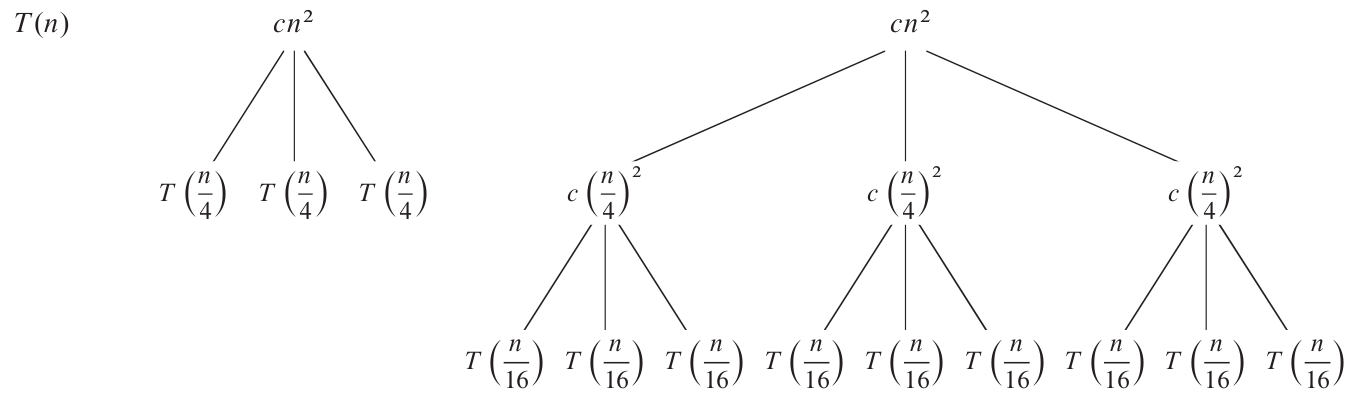
\includegraphics[width=1\textwidth]{figs/chap03/tree96-1}
\end{figure}
\end{itemize}
\end{frame}


\begin{frame}{‌روش درخت بازگشت}
\begin{itemize}\itemr
\item[-]
اگر مجموع هرینه‌ها را در هر سطح محاسبه کنیم، درختی با هزینه‌های قید شده در زیر خواهیم داشت.
\begin{figure}
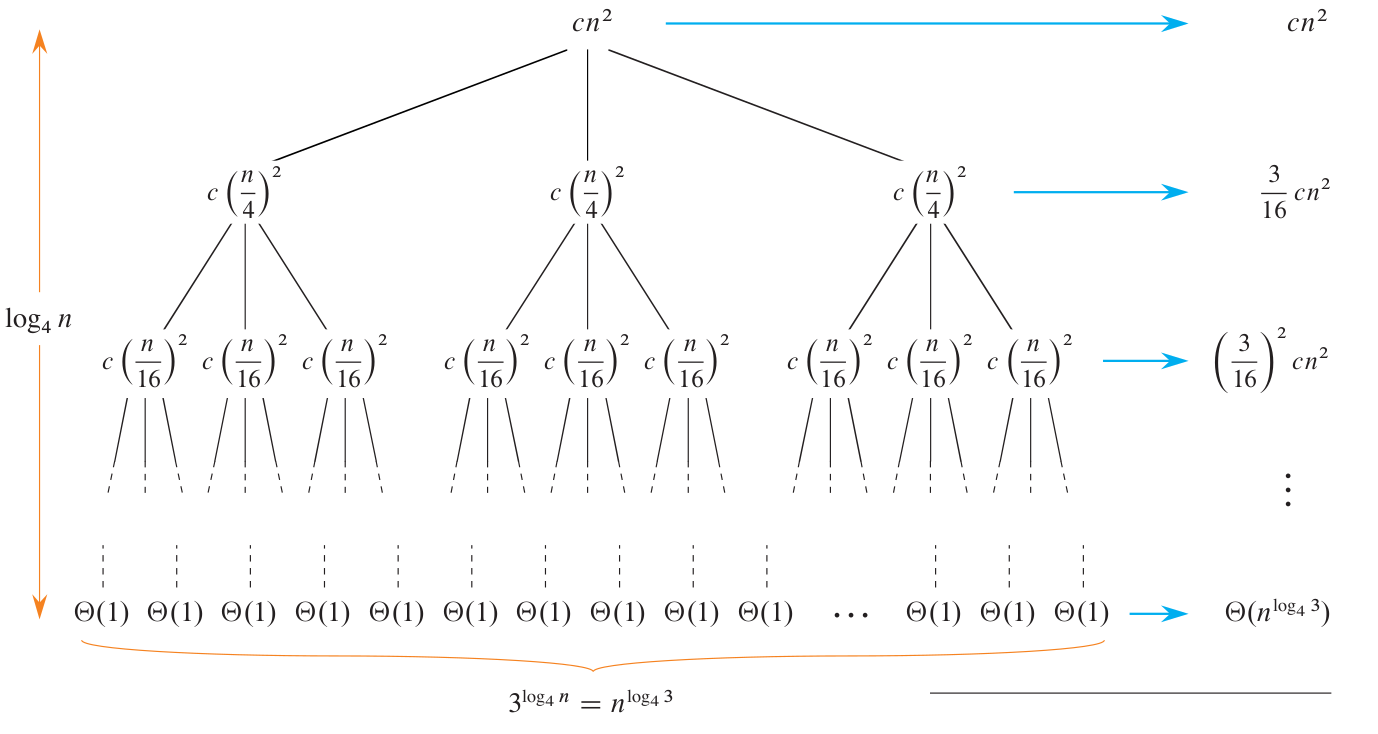
\includegraphics[width=0.9\textwidth]{figs/chap03/tree96-2}
\end{figure}
\end{itemize}
\end{frame}


\begin{frame}{‌روش درخت بازگشت}
\begin{itemize}\itemr
\item[-]
سپس هزینه‌های سطوح این درخت بازگشت را با هم جمع می‌کنیم و جواب رابطه بازگشتی را به دست می‌آوریم.
\end{itemize}
\end{frame}


\begin{frame}{‌روش درخت بازگشت}
\begin{itemize}\itemr
\item[-]
\begin{align*}
\m{T(n)} & \m{~= cn^2 + \frac{3}{16} cn^2 + {\left( \frac{3}{16} \right)}^2 cn^2 + \cdots +{\left( \frac{3}{16} \right)}^{\log_4 n} cn^2 + \ath {n^{\log_4 3}}}\\
& \m{~= {\sum_{i=0}^{\log_4 n}} {\left( \frac{3}{16} \right)}^i cn^2 + \ath {n^{\log_4 3}}} \\
& \m{~<  {\sum_{i=0}^{\infty}} {\left( \frac{3}{16} \right)}^i cn^2 + \ath {n^{\log_4 3}}}\\
& \m{~= \frac{1}{1 - (3/16)} cn^2 + \ath {n^{\log_4 3}}}\\
& \m{~= \frac{16}{13} cn^2 + \ath {n^{\log_4 3}}}\\
& \m{~= O(n^2)} ~~~~~~~~~~~~~~~~~~~~~~~~~~~~~~~~~~~ \m{(\ath {n^{\log_4 3}} = O(n^{0.8}) = O(n^2)).}
\end{align*}
\end{itemize}
\end{frame}


\begin{frame}{‌روش قضیه اصلی}
\begin{itemize}\itemr
\item[-]
روش قضیه اصلی
\fn{1}{master theorem method}
برای حل مسائل بازگشتی استفاده می‌شود که به صورت
\m{T(n) = aT(n/b) + f(n)}
هستند به طوری که
\m{a > 0}
و
\m{b > 1}
دو ثابت هستند.
\item[-]
تابع
\m{f(n)}
در اینجا تابع محرک
\fn{2}{driving function}
 نامیده می‌شود و یک رابطهٔ بازگشتی که به شکل مذکور است، رابطهٔ بازگشتی اصلی
\fn{3}{master recurrence}
  نامیده می‌شود.
\item[-]
در واقع رابطهٔ بازگشتی اصلی زمان اجرای الگوریتم‌های تقسیم و حل را توصیف می‌کند که مسئله‌ای به اندازهٔ n را به a زیر مسئله هر کدام با اندازهٔ
\m{n/b}
تقسیم می‌کنند. تابع
\m{f(n)}
هزینه تقسیم مسئله به زیر مسئله‌ها به علاوه هزینه ترکیب زیر مسئله‌ها را نشان می‌دهد.
\item[-]
اگر یک رابطهٔ بازگشتی شبیه رابطه قضیه اصلی باشد و علاوه بر آن چند عملگر کف و سقف در آن وجود داشته باشد، همچنان می‌توان از رابطهٔ قضیه اصلی استفاده کرد.
\end{itemize}
\end{frame}


\begin{frame}{‌روش قضیه اصلی}
\begin{itemize}\itemr
\item[-]
قضیه اصلی : فرض کنید
\m{a > 0}
و
\m{b > 1}
دو ثابت باشند و
\m{f(n)}
یک تابع باشد که برای اعداد بسیار بزرگ تعریف شده باشد.
\item[-]
رابطهٔ بازگشتی
\m{T(n)}
که بر روی اعداد طبیعی
\m{n \in \NN}
تعریف شده است را به صورت زیر در نظر بگیرید.
\begin{center}
\m{T(n) = aT(n/b) + f(n)}
\end{center}
\iffalse
به طوری که
\m{aT(n/b)}
برابر است با
\m{a'T( \lfloor n/b \rfloor ) + a"T(\lceil n/b \rceil)}
به ازای ثابت‌های
\m{a' \geqslant 0}
و
\m{a" \geqslant 0}
که در رابطهٔ
\m{a = a' + a"}
صدق می‌کنند.
\fi
\end{itemize}
\end{frame}


\begin{frame}{‌روش قضیه اصلی}
\begin{itemize}\itemr
\item[-]
 رفتار مجانبی
\m{T(n) = aT(n/b) + f(n)}
به صورت زیر است :
\item[۱-]
اگر ثابت
\m{\epsilon > 0}
وجود داشته باشد به طوری‌که
\m{f(n) = O(n^{\log_b^a - \epsilon})}
آنگاه
\m{T(n) = \ath{n^{\log_b^a}}}.
\item[۲-]
اگر ثابت
\m{k \geqslant 0}
وجود داشته باشد به طوری‌که
\m{f(n) = \ath{n^{\log_b^a} \lg^k n}}
آنگاه
\m{T(n) = \ath{n^{\log_b^a} \lg^{k+1}n}}.
\item[۳-]
اگر ثابت
\m{\epsilon > 0}
وجود داشته باشد به طوری‌که
\m{f(n) = \Omega(n^{\log_b^a + \epsilon})}
 آنگاه
\m{T(n) = \ath{f(n)}}.

برای برخی از توابع
\m{f(n)}
 نیاز داریم بررسی کنیم
\m{f(n)}
در رابطهٔ
\m{af(n/b) \leqslant cf(n)}
 به ازای
\m{c < 1}
و 
\m{n}
 های به اندازهٔ کافی بزرگ
صدق کند، اما برای توابعی که در تحلیل الگوریتم‌ها به آنها برمی‌خوریم این شرط معمولا برقرار است.
\end{itemize}
\end{frame}


\begin{frame}{‌روش قضیه اصلی}
\begin{itemize}\itemr
\item[۱-]
در حالت اول رشد جزء بازگشتی از رشد تابع محرک بیشتر است.
به عنوان مثال در
\m{T(n) = 2T(n/2) + \lg n}
رشد جزء بازگشتی
\ath{n}
و رشد تابع محرک
\ath{\lg n}
است.
بنابراین
\m{T(n) = \ath{n}} .
\item[۲-]
در حالت دوم رشد جزء بازگشتی و تابع محرک برابر است و یا رشد تابع محرک با یک ضریب
\ath{\lg^k n}
از جزء بازگشتی سریع‌تر است. به عنوان مثال در
\m{T(n) = 2T(n/2) + n \lg n}
رشد جزء بازگشتی
\ath{n}
و رشد تابع محرک
\ath{n \lg n}
است.
در این حالت تعداد سطوح درخت بازگشت 
\m{\lg n}
و مجموع هزینه‌های هر سطح
\ath{n \lg n}
است. بنابراین 
\m{T(n) = \ath{n \lg^2 n}} .
\item[۳-]
در حالت سوم رشد جزء بازگشتی از رشد تابع محرک کمتر است.
به عنوان مثال در
\m{T(n) = 2T(n/2) + n^2}
رشد جزء بازگشتی
\ath{n}
و رشد تابع محرک
\ath{n^2}
است.
بنابراین
\m{T(n) = \ath{n^2}} .
\end{itemize}
\end{frame}


\begin{frame}{‌روش قضیه اصلی}
\begin{itemize}\itemr
\item[-]
در یک حالت خاص اگر داشته باشیم، 
\m{T(n) = aT(n/b) + cn^k}
آنگاه می‌توانیم اثبات کنیم:
\begin{align*}
\m{T(n)} = \left\{\begin{array}{lr}
          \m{\Theta(n^{\log_b a})}& \m{a > b^k}~\text{اگر}\\
          \m{\Theta(n^k \lg n)}& \m{a = b^k}~\text{اگر}\\
          \m{\Theta(n^k)}& \m{a < b^k}~\text{اگر}
\end{array}\right.
\end{align*}

\end{itemize}
\end{frame}

\begin{frame}{‌روش قضیه اصلی}
\begin{itemize}\itemr
\item[-]
رابطهٔ بازگشتی
\m{T(n) = 9T(n/3) + n}
را در نظر بگیرید. در این رابطه داریم
\m{a = 9}
و
\m{b = 3}
بنابراین به دست می‌آوریم
\m{n^{\log_b^a} = n^{\log_3^9} = \ath{n^2}}.
از آنجایی که
\m{f(n) = n = O(n^{2- \epsilon})}
به ازای هر ثابت
\m{\epsilon < 1}
بنابراین می‌توانیم حالت اول در قضیه اصلی را در نظر بگیریم و نتیجه بگیریم
\m{T(n) = \ath{n^2}}.
\end{itemize}
\end{frame}


\begin{frame}{‌روش قضیه اصلی}
\begin{itemize}\itemr
\item[-]
رابطهٔ بازگشتی
\m{T(n) = T(2n/3) + 1}
را در نظر بگیرید. در این رابطه داریم
\m{a = 1}
و
\m{b = 3/2}
بنابراین
\m{n^{\log_b^a} = n^{\log_{3/2}^1} = n^0 = 1}.
در اینجا حالت دوم در قضیه اصلی را داریم یعنی
\m{f(n) = 1 = \ath{n^{\log_b^a} \lg^0 n} = \ath{1}}
بنابراین جواب رابطهٔ بازگشتی برابر است با
\m{T(n) = \ath{\lg n}}.
\end{itemize}
\end{frame}


\begin{frame}{‌روش قضیه اصلی}
\begin{itemize}\itemr
\item[-]
در رابطهٔ بازگشتی
\m{T(n) = 3T(n/4) + n\lg n}
داریم
\m{a = 3}
و
\m{b = 4}
که بدین معنی است که
\m{n^{\log_b^a} = n^{\log_4^3} = \ath{n^{0.793}}}.
از آنجایی که
\m{f(n) = n \lg n = \Omega (n^{\log_4^3 + \epsilon})}
جایی که
\m{\epsilon}
حدود
\m{0.2}
است، بنابراین حالت سوم در قضیه اصلی را می‌توانیم در نظر بگیریم اگر شرط
\m{af(n/b) \leqslant cf(n)}
برقرار باشد.
\begin{flushleft}
\m{af(n/b) = 3(n/4) \lg(n/4) \leqslant (3/4) n \lg n = 3/4f(n)}
\end{flushleft}
بنابراین با استفاده از حالت سوم جواب رابطهٔ بازگشتی برابراست با
\m{T(n) = \ath{n \lg n}}.
\end{itemize}
\end{frame}


\begin{frame}{‌روش قضیه اصلی}
\begin{itemize}\itemr
\item[-]
رابطهٔ بازگشتی
\m{T(n) = 2T(n/2) + \ath{n}}
رابطه‌ای بود که برای مرتب‌سازی ادغامی به دست آوردیم. از آنجایی که
\m{a = 2}
و
\m{b = 2}
داریم
\m{n^{\log_2^2} = n}.
حالت دوم در اینجا برقراراست زیرا به ازای
\m{k=0}
داریم
\m{f(n) = \ath{n}}
و بنابراین جواب رابطهٔ بازگشتی برابر است با
\m{T(n) = \ath{n \lg n}}.
\end{itemize}
\end{frame}


\begin{frame}{‌روش قضیه اصلی}
\begin{itemize}\itemr
\item[-]
رابطهٔ
\m{T(n) = 8T(n/2) + \ath{1}}
زمان اجرای الگوریتم ضرب ماتریسی را توصیف می‌کند. در اینجا داریم
\m{a = 8}
و
\m{b = 2}
بنابراین
\m{n^{\log_2^8} = n^3}.
تابع محرک
\m{f(n) = \ath{1}}
 است و بنابراین به ازای هر
\m{ \epsilon < 3}
داریم
\m{f(n) = O(n^{3 - \epsilon})} .
بنابراین حالت اول قضیه اصلی برقرار است. نتیجه می‌گیریم
\m{T(n) = \ath{n^3}}.
\end{itemize}
\end{frame}


\begin{frame}{‌روش قضیه اصلی}
\begin{itemize}\itemr
\item[-]
در تحلیل زمان اجرای الگوریتم استراسن رابطهٔ
\m{T(n) = 7T(n/2) + \ath{n^2}}
را به دست آوردیم. در این رابطهٔ بازگشتی
\m{a = 7}
و
\m{b = 2}
بنابراین
\m{n^{\log_2^7} = n^{\lg 7}}.
از آنجایی که
\m{\lg 7 = 2.8073...}
، می‌توانیم قرار دهیم
\m{\epsilon = 0.8}
و برای تابع محرک خواهیم داشت
\m{f(n) = \ath{n^2} = O \bigl( n^{\lg 7 - \epsilon} \bigr)}
، پس حالت اول در قضیه اصلی برقرار است و بنابراین جواب رابطهٔ بازگشتی برابر است با
\m{T(n) = \ath{n^{\lg 7}}}.
\end{itemize}
\end{frame}


%%%%%%%%%%%%

%%%%%%%%%%%%
%\section*{References}
%\begin{frame}<0>[noframenumbering]
%\bibliographystyle{apalike}
%\bibliography{docs/bib}
%\end{frame}
%%%%%%%%%%%%

\end{document}
